% ============================================================================
% CVE2 RISC-V PROCESSOR IMPLEMENTATION ON LATTICE ECP5-5G FPGA
% Research Paper - Part 1: Document Setup and Introduction
% Author: Kaushal
% Date: November 5, 2025
% ============================================================================

\documentclass[12pt,a4paper]{article}

% ============================================================================
% PACKAGES
% ============================================================================
\usepackage[utf8]{inputenc}
\usepackage[T1]{fontenc}
\usepackage{geometry}
\geometry{a4paper, margin=1in}

% Typography and fonts
\usepackage{times}
\usepackage{microtype}
\usepackage{setspace}
\onehalfspacing

% Mathematics
\usepackage{amsmath}
\usepackage{amssymb}
\usepackage{amsfonts}

% Graphics and figures
\usepackage{graphicx}
\usepackage{float}
\usepackage{subfig}
\usepackage{tikz}
\usetikzlibrary{shapes,arrows,positioning,calc,circuits.logic.US}

% Tables
\usepackage{booktabs}
\usepackage{multirow}
\usepackage{longtable}
\usepackage{array}

% Code listings
\usepackage{listings}
\usepackage{xcolor}

% Hyperlinks and references
\usepackage{hyperref}
\hypersetup{
    colorlinks=true,
    linkcolor=blue,
    filecolor=magenta,      
    urlcolor=cyan,
    citecolor=green,
    pdftitle={CVE2 RISC-V Processor Implementation on ECP5-5G FPGA},
    pdfauthor={Kaushal},
    pdfsubject={RISC-V Processor Implementation, FPGA Design, Open-Source Toolchain},
    pdfkeywords={RISC-V, CVE2, FPGA, ECP5, Open-Source Tools, sv2v, Yosys, nextpnr}
}

% Headers and footers
\usepackage{fancyhdr}
\pagestyle{fancy}
\fancyhf{}
\fancyhead[L]{\leftmark}
\fancyhead[R]{\thepage}
\renewcommand{\headrulewidth}{0.4pt}
\setlength{\headheight}{14.5pt}

% Code listing style configuration
\definecolor{codegreen}{rgb}{0,0.6,0}
\definecolor{codegray}{rgb}{0.5,0.5,0.5}
\definecolor{codepurple}{rgb}{0.58,0,0.82}
\definecolor{backcolour}{rgb}{0.95,0.95,0.92}
\definecolor{verilogblue}{rgb}{0.0,0.0,0.8}

\lstdefinestyle{verilogstyle}{
    backgroundcolor=\color{backcolour},   
    commentstyle=\color{codegreen},
    keywordstyle=\color{verilogblue}\bfseries,
    numberstyle=\tiny\color{codegray},
    stringstyle=\color{codepurple},
    basicstyle=\ttfamily\footnotesize,
    breakatwhitespace=false,         
    breaklines=true,                 
    captionpos=b,                    
    keepspaces=true,                 
    numbers=left,                    
    numbersep=5pt,                  
    showspaces=false,                
    showstringspaces=false,
    showtabs=false,                  
    tabsize=4,
    frame=single,
    rulecolor=\color{black},
    language=Verilog
}

\lstdefinestyle{bashstyle}{
    backgroundcolor=\color{black!5},   
    commentstyle=\color{codegreen},
    keywordstyle=\color{blue}\bfseries,
    numberstyle=\tiny\color{codegray},
    stringstyle=\color{codepurple},
    basicstyle=\ttfamily\footnotesize,
    breakatwhitespace=false,         
    breaklines=true,                 
    captionpos=b,                    
    keepspaces=true,                 
    numbers=none,                    
    showspaces=false,                
    showstringspaces=false,
    showtabs=false,                  
    tabsize=4,
    frame=leftline,
    framerule=2pt,
    rulecolor=\color{gray}
}

\lstdefinestyle{assemblystyle}{
    backgroundcolor=\color{white},   
    commentstyle=\color{codegreen},
    keywordstyle=\color{blue}\bfseries,
    numberstyle=\tiny\color{codegray},
    basicstyle=\ttfamily\footnotesize,
    breaklines=true,                 
    captionpos=b,                    
    keepspaces=true,                 
    numbers=left,                    
    showspaces=false,                
    showstringspaces=false,
    showtabs=false,                  
    tabsize=4,
    frame=single,
    rulecolor=\color{black}
}

\lstset{style=verilogstyle}

% Custom commands
\newcommand{\code}[1]{\texttt{#1}}
\newcommand{\file}[1]{\texttt{\textbf{#1}}}
\newcommand{\cmd}[1]{\texttt{\$ #1}}

% Title information
\title{
    \vspace{-1cm}
    {\LARGE\bfseries Implementation of OpenHW Group CVE2 RISC-V Processor on Lattice ECP5-5G FPGA} \\
    \vspace{0.5cm}
    {\Large A Complete Guide to Open-Source RISC-V SoC Design Using SystemVerilog-to-Verilog Flow}
}

\author{
    Kaushal \\
    \textit{Btech in EE @ IITdh} \\
    \texttt{kaushal@riscv.fpga.dev}
}

\date{November 5, 2025}

% ============================================================================
% DOCUMENT BEGINS
% ============================================================================
\begin{document}

\maketitle

\begin{abstract}
This paper presents a comprehensive implementation of the OpenHW Group CVE2 RISC-V processor on a Lattice ECP5-5G Field-Programmable Gate Array (FPGA) using an entirely open-source toolchain. The CVE2 core, a 32-bit in-order RISC-V processor written in SystemVerilog, is integrated into a minimal System-on-Chip (SoC) architecture featuring 8KB of internal RAM and memory-mapped GPIO peripherals.

The implementation workflow employs sv2v for SystemVerilog-to-Verilog conversion, Yosys for logic synthesis, nextpnr-ecp5 for place-and-route, ecppack for bitstream generation, and OpenOCD for JTAG programming. The design targets the ECP5-5G Versa Development Kit and successfully demonstrates processor execution through an 8-bit counter program driving the board's LED array.

This work addresses critical challenges in FPGA-based RISC-V implementation including: (1) SystemVerilog language subset compatibility for open-source synthesis, (2) FPGA-safe clock gating replacement, (3) instruction memory interface protocol alignment, (4) active-low I/O polarity management, and (5) timing closure optimization through architectural tuning.

Resource utilization analysis shows the configured CVE2 core (RV32E with no multiplication extension) consumes 26,037 LUT4s (59\% of available logic), 1,359 flip-flops (3\%), and 2,048 distributed RAM cells (37\% of LUT-RAM capacity) on the LFE5UM5G-45F device. The design achieves timing closure at 40.79 MHz for the CPU clock domain, significantly exceeding the target frequency derived from the 100 MHz board oscillator.

The complete project demonstrates end-to-end RISC-V processor deployment on FPGAs without proprietary vendor tools, providing a reproducible reference for open-source hardware development, computer architecture education, and RISC-V ecosystem advancement.

\textbf{Keywords:} RISC-V, CVE2, FPGA, ECP5, SystemVerilog, Open-Source EDA, sv2v, Yosys, nextpnr, SoC Design, Hardware/Software Co-Design
\end{abstract}

\newpage
\tableofcontents
\newpage

% ============================================================================
% SECTION 1: INTRODUCTION
% ============================================================================
\section{Introduction}

\subsection{Motivation and Context}

The RISC-V Instruction Set Architecture (ISA) represents a paradigm shift in processor design, offering a free and open standard that eliminates the licensing constraints, fragmentation, and vendor lock-in that have historically characterized the semiconductor industry. Unlike proprietary architectures such as ARM or x86, RISC-V provides a modular, extensible ISA specification that enables innovation at all levels of the computing stack—from embedded microcontrollers to high-performance server processors.

Field-Programmable Gate Arrays (FPGAs) serve as an ideal platform for RISC-V processor implementation, prototyping, and research. FPGAs provide:

\begin{itemize}
    \item \textbf{Rapid prototyping}: Immediate hardware iteration without fabrication delays
    \item \textbf{Architectural exploration}: Easy evaluation of microarchitectural trade-offs
    \item \textbf{Custom extensions}: Implementation of domain-specific RISC-V instructions
    \item \textbf{Educational value}: Hands-on learning of processor design principles
    \item \textbf{Verification platform}: Hardware-in-the-loop testing before ASIC tape-out
\end{itemize}

The convergence of open-source RISC-V processors and open-source FPGA toolchains democratizes processor design, enabling researchers, educators, and engineers worldwide to experiment with and contribute to cutting-edge computer architecture without expensive commercial EDA (Electronic Design Automation) software.

\subsection{Project Objectives}

This work aims to achieve the following objectives:

\begin{enumerate}
    \item \textbf{Implement CVE2 RISC-V Core}: Deploy the OpenHW Group CVE2 processor (a 32-bit, 2-stage pipeline, RV32IMC-capable core) on Lattice ECP5-5G FPGA hardware.
    
    \item \textbf{Utilize Open-Source Toolchain}: Demonstrate complete FPGA development flow using only freely-available, open-source tools (sv2v, Yosys, nextpnr, Project Trellis, OpenOCD).
    
    \item \textbf{Design Minimal SoC}: Create a functional System-on-Chip with internal memory, memory-mapped I/O, and proper bus interface protocols.
    
    \item \textbf{Verify Operation}: Prove correct processor execution through firmware execution that produces visible output on physical hardware (LED array).
    
    \item \textbf{Document Methodology}: Provide comprehensive, reproducible documentation of the entire design flow from RTL to bitstream programming.
    
    \item \textbf{Analyze Results}: Present detailed resource utilization, timing analysis, and design optimization insights.
    
    \item \textbf{Address Challenges}: Document solutions to SystemVerilog synthesis limitations, clock gating incompatibilities, and interface protocol mismatches.
\end{enumerate}

\subsection{CVE2 Processor Overview}

\subsubsection{Core Architecture}

The CVE2 (pronounced "CV-E-two") is a small, efficient, 32-bit RISC-V processor designed by the OpenHW Group's CORE-V project. Key architectural features include:

\begin{itemize}
    \item \textbf{ISA Support}: RV32I base integer instruction set with optional M (multiplication), C (compressed instructions), and E (embedded/reduced registers) extensions
    
    \item \textbf{Pipeline}: 2-stage pipeline (Instruction Fetch, Execute) optimized for low latency and minimal area
    
    \item \textbf{Core-V Extensions}: Support for CORE-V eXtension Interface (X-Interface) for custom instructions
    
    \item \textbf{Privilege Modes}: Machine mode (M-mode) with optional User mode support
    
    \item \textbf{CSRs}: Standard Control and Status Registers for interrupts, exceptions, and performance counters
    
    \item \textbf{Interrupts}: CLINT-compatible timer and software interrupts, PLIC-compatible external interrupts
    
    \item \textbf{Debug Support}: RISC-V External Debug specification compliance
\end{itemize}

\subsubsection{Microarchitecture Highlights}

\textbf{Instruction Fetch (IF) Stage:}
\begin{itemize}
    \item Request-grant handshake protocol for memory interface
    \item Prefetch buffer for improved throughput
    \item Branch predictor (optional, not implemented in minimal configuration)
\end{itemize}

\textbf{Execute (EX) Stage:}
\begin{itemize}
    \item ALU operations (arithmetic, logical, shifts)
    \item Branch/jump target calculation
    \item Load/Store address generation
    \item CSR access and exception handling
\end{itemize}

\textbf{Register File:}
\begin{itemize}
    \item 32 general-purpose registers (x0-x31) for RV32I
    \item 16 registers (x0-x15) for RV32E (embedded configuration)
    \item Dual-port read, single-port write
\end{itemize}

\subsubsection{CVE2 vs. Other RISC-V Cores}

Comparison with popular open-source RISC-V cores:

\begin{table}[H]
\centering
\caption{RISC-V Core Comparison}
\label{tab:riscv_comparison}
\begin{tabular}{@{}lllll@{}}
\toprule
\textbf{Feature} & \textbf{CVE2} & \textbf{Ibex} & \textbf{PicoRV32} & \textbf{VexRiscv} \\
\midrule
Pipeline Stages & 2 & 2 & 1 (multi-cycle) & 5 (configurable) \\
ISA & RV32IMC/E & RV32IMC/E & RV32IMC & RV32IM \\
Area (gates) & \textasciitilde25K & \textasciitilde30K & \textasciitilde15K & \textasciitilde40K \\
Max Freq (ASIC) & 400+ MHz & 450+ MHz & 250 MHz & 300+ MHz \\
Language & SystemVerilog & SystemVerilog & Verilog & SpinalHDL \\
Organization & OpenHW Group & lowRISC & Clifford Wolf & Charles Papon \\
\bottomrule
\end{tabular}
\end{table}

CVE2 occupies a sweet spot between PicoRV32's minimalism and VexRiscv's complexity, offering good performance-per-area while maintaining synthesis compatibility.

\subsection{ECP5-5G Target Platform}

\subsubsection{Lattice ECP5 FPGA Family}

The Lattice ECP5 family offers:
\begin{itemize}
    \item \textbf{Logic capacity}: 12K to 85K LUT4s
    \item \textbf{Embedded memory}: Up to 3.7 Mb block RAM
    \item \textbf{DSP blocks}: 18x18 multipliers
    \item \textbf{SerDes}: 5 Gbps SERDES channels (5G variants)
    \item \textbf{Power efficiency}: Excellent mW/LUT ratio
\end{itemize}

Our target device: \textbf{LFE5UM5G-45F-8BG381C}
\begin{itemize}
    \item 43,848 LUT4s (45K nominal)
    \item 1,008 Kb embedded block RAM
    \item 197 user I/O pins
    \item 381-ball BGA package
    \item Speed grade 8 (fastest)
\end{itemize}

\subsubsection{ECP5-5G Versa Development Board}

The Versa evaluation platform provides:
\begin{itemize}
    \item Central LFE5UM5G-45F FPGA
    \item 100 MHz LVDS differential clock oscillator
    \item 8 user LEDs (active-low configuration)
    \item 14-segment alphanumeric display
    \item FTDI FT2232H USB-JTAG interface
    \item Rich connectivity (Ethernet, PCIe, HDMI, expansion headers)
    \item On-board SPI Flash for configuration storage
\end{itemize}

\textbf{Clock Source Details:}
\begin{itemize}
    \item Frequency: 100.000 MHz $\pm$ 50 ppm
    \item Standard: LVDS (Low-Voltage Differential Signaling)
    \item FPGA Pin: P3 (differential pair P3/N3)
    \item Period: $T = 10$ ns
\end{itemize}

\subsection{Open-Source FPGA Toolchain}

\subsubsection{Tool Components}

The complete open-source flow comprises:

\begin{description}
    \item[sv2v] SystemVerilog-to-Verilog conversion tool by Zachary Snow. Translates synthesizable SystemVerilog to pure Verilog-2005, enabling use with Yosys.
    
    \item[Yosys] Open-source synthesis framework by Claire Xen (formerly Clifford Wolf). Performs RTL elaboration, logic optimization, technology mapping, and netlist generation.
    
    \item[nextpnr] Portable FPGA place-and-route tool. Implements the synthesized netlist onto specific FPGA architectures using analytical placement and routing algorithms.
    
    \item[Project Trellis] Lattice ECP5 bitstream documentation and tooling. Provides the architectural database (chip DB) for nextpnr and bitstream assembly tools.
    
    \item[ecppack] Bitstream assembly tool (part of Trellis). Converts placed-and-routed design into FPGA configuration bitstream (.bit) and Serial Vector Format (.svf) for programming.
    
    \item[OpenOCD] Open On-Chip Debugger. Provides JTAG interface for bitstream download, boundary scan, and debug access.
\end{description}

\subsubsection{Tool Flow Overview}

\begin{figure}[H]
\centering
\begin{tikzpicture}[
    node distance=1.2cm,
    process/.style={rectangle, draw, fill=blue!20, text width=4cm, text centered, rounded corners, minimum height=1cm},
    file/.style={rectangle, draw, fill=green!20, text width=3.5cm, text centered, minimum height=0.8cm},
    arrow/.style={->, >=stealth, thick}
]

\node[file] (sv) {SystemVerilog RTL\\(cve2\_*.sv)};
\node[process, below=of sv] (sv2v) {sv2v\\SV → Verilog Conversion};
\node[file, below=of sv2v] (v) {Verilog Netlist\\(cve2\_*.v)};
\node[process, below=of v] (yosys) {Yosys\\Logic Synthesis};
\node[file, below=of yosys] (json) {JSON Netlist\\(design.json)};
\node[process, below=of json] (nextpnr) {nextpnr-ecp5\\Place \& Route};
\node[file, below=of nextpnr] (config) {Textual Config\\(design\_out.config)};
\node[process, below=of config] (ecppack) {ecppack\\Bitstream Assembly};
\node[file, below=of ecppack] (bit) {Bitstream\\(design.bit, .svf)};
\node[process, below=of bit] (openocd) {OpenOCD\\JTAG Programming};
\node[file, below=of openocd] (fpga) {Configured FPGA};

\draw[arrow] (sv) -- (sv2v);
\draw[arrow] (sv2v) -- (v);
\draw[arrow] (v) -- (yosys);
\draw[arrow] (yosys) -- (json);
\draw[arrow] (json) -- (nextpnr);
\draw[arrow] (nextpnr) -- (config);
\draw[arrow] (config) -- (ecppack);
\draw[arrow] (ecppack) -- (bit);
\draw[arrow] (bit) -- (openocd);
\draw[arrow] (openocd) -- (fpga);

\end{tikzpicture}
\caption{Open-Source FPGA Design Flow}
\label{fig:toolflow}
\end{figure}

\subsection{Related Work}

\subsubsection{RISC-V on FPGAs}

Previous implementations of RISC-V processors on FPGAs include:

\begin{itemize}
    \item \textbf{SiFive Freedom E310}: Commercial RISC-V core on Xilinx FPGAs
    \item \textbf{PicoRV32 on iCE40}: Clifford Wolf's minimal implementation
    \item \textbf{NEORV32}: Full-featured SoC on Intel and Xilinx devices
    \item \textbf{Ibex on various platforms}: lowRISC's educational core
\end{itemize}

This work distinguishes itself by targeting the ECP5 platform with the CVE2 core using exclusively open-source tools.

\subsubsection{Open-Source FPGA Tools Evolution}

Key milestones in open-source FPGA development:
\begin{itemize}
    \item 2015: IceStorm project reverse-engineers Lattice iCE40 bitstream
    \item 2016: Yosys synthesis flow matures
    \item 2018: nextpnr released as portable place-and-route tool
    \item 2018: Project Trellis documents ECP5 architecture
    \item 2020+: sv2v enables SystemVerilog compatibility
\end{itemize}

\subsection{Document Organization}

The remainder of this paper is structured as follows:

\begin{description}
    \item[Section 2] \textbf{Background and Theory}: Detailed coverage of RISC-V ISA, processor microarchitecture, FPGA architecture, and synthesis/P\&R algorithms.
    
    \item[Section 3] \textbf{System Architecture}: Description of the CVE2 SoC design including memory map, bus interfaces, GPIO peripherals, and firmware embedding.
    
    \item[Section 4] \textbf{Implementation Methodology}: Step-by-step design flow from RTL acquisition through bitstream generation, including all tool invocations and parameters.
    
    \item[Section 5] \textbf{Critical Design Challenges}: Analysis of and solutions to: SystemVerilog synthesis issues, clock gating incompatibility, instruction interface protocol, and I/O polarity.
    
    \item[Section 6] \textbf{Build Optimization}: Techniques for accelerating P\&R including multi-threading, core size reduction, and quick reprogram workflow.
    
    \item[Section 7] \textbf{Results and Analysis}: Resource utilization tables, timing reports, verification procedures, and performance metrics.
    
    \item[Section 8] \textbf{Discussion}: Design trade-offs, lessons learned, and comparison with alternative approaches.
    
    \item[Section 9] \textbf{Conclusion and Future Work}: Summary of contributions and directions for extension.
    
    \item[Appendices] Complete source code listings, constraint files, and build scripts.
\end{description}

\subsection{Contributions}

This work makes the following contributions:

\begin{enumerate}
    \item \textbf{Complete open-source CVE2 implementation}: First documented end-to-end deployment of CVE2 processor on ECP5 using only FOSS tools.
    
    \item \textbf{SystemVerilog synthesis methodology}: Demonstration of sv2v workflow for complex RTL with packages, interfaces, and parameterization.
    
    \item \textbf{FPGA-specific adaptations}: Solutions to simulation-only constructs (clock gating) and protocol mismatches (instruction interface).
    
    \item \textbf{Reproducible documentation}: Complete artifact preservation enabling replication by other researchers and engineers.
    
    \item \textbf{Educational resource}: Detailed explanations suitable for students learning processor design and FPGA implementation.
\end{enumerate}
% ============================================================================
% PART 2: BACKGROUND AND THEORY
% This file continues the CVE2 RISC-V paper
% ============================================================================

% ============================================================================
% SECTION 2: BACKGROUND AND THEORY
% ============================================================================
\section{Background and Theory}

\subsection{RISC-V Instruction Set Architecture}

\subsubsection{ISA Philosophy and Design Principles}

The RISC-V ISA embodies five decades of computer architecture research, distilling lessons from RISC I, MIPS, ARM, and other processor designs into a clean, modular specification. Core design principles include:

\begin{itemize}
    \item \textbf{Simplicity}: Minimal base ISA with optional extensions
    \item \textbf{Modularity}: Cleanly separated features (I, M, A, F, D, C extensions)
    \item \textbf{Extensibility}: Custom instruction space for domain-specific acceleration
    \item \textbf{Stability}: Frozen base ISA ensures long-term software compatibility
    \item \textbf{Privilege levels}: Machine, Supervisor, User modes for security
\end{itemize}

\subsubsection{RV32I Base Integer Instruction Set}

The RV32I base ISA defines 47 instructions across six categories:

\textbf{1. Integer Computational Instructions:}
\begin{itemize}
    \item Arithmetic: ADD, SUB, ADDI
    \item Logical: AND, OR, XOR, ANDI, ORI, XORI
    \item Shifts: SLL, SRL, SRA, SLLI, SRLI, SRAI
    \item Comparisons: SLT, SLTU, SLTI, SLTIU
    \item Upper immediate: LUI, AUIPC
\end{itemize}

\textbf{2. Control Transfer Instructions:}
\begin{itemize}
    \item Unconditional jumps: JAL (jump and link), JALR (jump and link register)
    \item Conditional branches: BEQ, BNE, BLT, BGE, BLTU, BGEU
\end{itemize}

\textbf{3. Load and Store Instructions:}
\begin{itemize}
    \item Loads: LB, LH, LW, LBU, LHU (byte, halfword, word; signed/unsigned)
    \item Stores: SB, SH, SW
\end{itemize}

\textbf{4. Memory Ordering:}
\begin{itemize}
    \item FENCE: Memory barrier for ordering loads/stores
\end{itemize}

\textbf{5. Control and Status Registers (CSR):}
\begin{itemize}
    \item CSRRW, CSRRS, CSRRC (read-write, read-set, read-clear)
    \item CSRRWI, CSRRSI, CSRRCI (immediate variants)
\end{itemize}

\textbf{6. System Instructions:}
\begin{itemize}
    \item ECALL: Environment call (system call)
    \item EBREAK: Breakpoint for debuggers
\end{itemize}

\subsubsection{Instruction Encoding}

RISC-V uses a fixed 32-bit instruction format with six major encoding types:

\begin{table}[H]
\centering
\caption{RISC-V Instruction Formats}
\label{tab:riscv_formats}
\small
\begin{tabular}{@{}llp{8cm}@{}}
\toprule
\textbf{Type} & \textbf{Fields} & \textbf{Usage} \\
\midrule
R-type & funct7|rs2|rs1|funct3|rd|opcode & Register-register operations (ADD, SUB, AND, OR) \\
I-type & imm[11:0]|rs1|funct3|rd|opcode & Immediate operations (ADDI), loads (LW), JALR \\
S-type & imm[11:5]|rs2|rs1|funct3|imm[4:0]|opcode & Stores (SW, SH, SB) \\
B-type & imm[12,10:5]|rs2|rs1|funct3|imm[4:1,11]|opcode & Conditional branches (BEQ, BNE) \\
U-type & imm[31:12]|rd|opcode & Upper immediate (LUI, AUIPC) \\
J-type & imm[20,10:1,11,19:12]|rd|opcode & Jump (JAL) \\
\bottomrule
\end{tabular}
\end{table}

Example instruction encoding for \code{ADDI x1, x0, 42}:
\begin{verbatim}
Binary:  000000101010 00000 000 00001 0010011
Hex:     0x02A00093
Fields:  imm=42 | rs1=x0 | funct3=0 | rd=x1 | opcode=0x13
\end{verbatim}

\subsubsection{RV32E: Embedded Extension}

The RV32E extension reduces the register file from 32 to 16 registers (x0-x15), trading programmer convenience for reduced hardware area:

\textbf{Benefits:}
\begin{itemize}
    \item Smaller register file: 50\% reduction in flip-flops
    \item Faster context switching: Fewer registers to save/restore
    \item Area-optimized for embedded systems
\end{itemize}

\textbf{Trade-offs:}
\begin{itemize}
    \item More register spilling to memory
    \item Reduced performance on register-intensive workloads
    \item Binary incompatibility with RV32I (different ABI)
\end{itemize}

In our implementation, we configured CVE2 with RV32E to accelerate place-and-route by reducing logic utilization.

\subsubsection{M Extension: Integer Multiplication and Division}

The M extension adds eight instructions:
\begin{itemize}
    \item MUL, MULH, MULHSU, MULHU: Multiplication with various signedness
    \item DIV, DIVU: Signed/unsigned division
    \item REM, REMU: Signed/unsigned remainder
\end{itemize}

CVE2 supports three M extension configurations:
\begin{itemize}
    \item \textbf{RV32MNone}: No multiplication/division (our choice for minimal area)
    \item \textbf{RV32MSlow}: Multi-cycle iterative implementation
    \item \textbf{RV32MFast}: Single-cycle with hardware multiplier
\end{itemize}

\subsection{CVE2 Microarchitecture}

\subsubsection{Pipeline Structure}

CVE2 implements a 2-stage pipeline optimized for low latency and minimal area:

\begin{figure}[H]
\centering
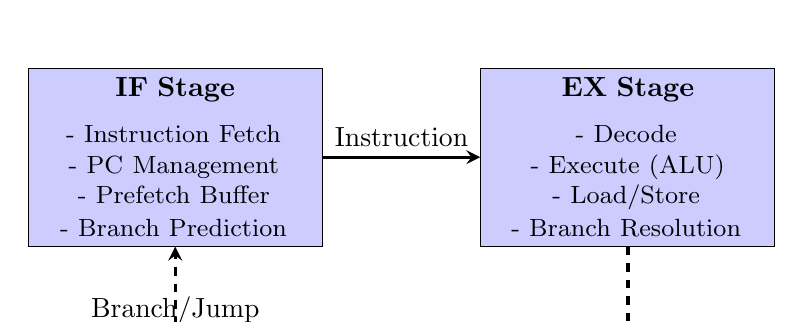
\begin{tikzpicture}[
    stage/.style={rectangle, draw, fill=blue!20, text width=3.5cm, text centered, minimum height=2cm},
    arrow/.style={->, >=stealth, very thick}
]

\node[stage] (if) {
    \textbf{IF Stage} \\[0.2cm]
    \small
    - Instruction Fetch \\
    - PC Management \\
    - Prefetch Buffer \\
    - Branch Prediction
};

\node[stage, right=2cm of if] (ex) {
    \textbf{EX Stage} \\[0.2cm]
    \small
    - Decode \\
    - Execute (ALU) \\
    - Load/Store \\
    - Branch Resolution
};

\draw[arrow] (if) -- (ex) node[midway, above] {Instruction};
\draw[arrow, dashed] (ex.south) -- ++(0,-1) -| (if.south) node[near end, below] {Branch/Jump};

\end{tikzpicture}
\caption{CVE2 Two-Stage Pipeline}
\label{fig:cve2_pipeline}
\end{figure}

\textbf{IF Stage Operations:}
\begin{enumerate}
    \item Assert \code{instr\_req\_o} to request instruction
    \item Wait for \code{instr\_gnt\_i} grant from memory
    \item Wait for \code{instr\_rvalid\_i} indicating data valid
    \item Read instruction from \code{instr\_rdata\_i}
    \item Increment or update PC based on control flow
\end{enumerate}

\textbf{EX Stage Operations:}
\begin{enumerate}
    \item Decode instruction opcode and operands
    \item Read register file (up to 2 source registers)
    \item Perform ALU operation or address calculation
    \item Access data memory if load/store
    \item Write result to register file (if applicable)
    \item Update PC for branches/jumps
\end{enumerate}

\subsubsection{Memory Interfaces}

CVE2 uses a simple request-grant handshake protocol for both instruction and data memory:

\textbf{Instruction Interface Signals:}
\begin{lstlisting}[style=verilogstyle, caption={Instruction Memory Interface}]
output logic        instr_req_o,      // Request valid
input  logic        instr_gnt_i,      // Grant (can accept req)
input  logic        instr_rvalid_i,   // Response valid
output logic [31:0] instr_addr_o,     // Address
input  logic [31:0] instr_rdata_i,    // Read data
input  logic        instr_err_i       // Error flag
\end{lstlisting}

\textbf{Data Interface Signals:}
\begin{lstlisting}[style=verilogstyle, caption={Data Memory Interface}]
output logic        data_req_o,       // Request valid
input  logic        data_gnt_i,       // Grant
input  logic        data_rvalid_i,    // Response valid
output logic        data_we_o,        // Write enable
output logic [3:0]  data_be_o,        // Byte enable
output logic [31:0] data_addr_o,      // Address
output logic [31:0] data_wdata_o,     // Write data
input  logic [31:0] data_rdata_i,     // Read data
input  logic        data_err_i        // Error flag
\end{lstlisting}

\textbf{Protocol Timing Diagram:}

\begin{verbatim}
Clock:      __|‾‾|__|‾‾|__|‾‾|__|‾‾|__|‾‾|__
req_o:      ______|‾‾‾‾‾‾‾‾‾‾‾|_________
gnt_i:      _________|‾‾‾‾‾|_____________
rvalid_i:   ______________|‾‾‾‾‾|________
rdata_i:    ==============<DATA>==========
\end{verbatim}

\textbf{Key Protocol Requirements:}
\begin{itemize}
    \item \code{gnt\_i} indicates the memory subsystem accepted the request
    \item \code{rvalid\_i} arrives one or more cycles later with valid data
    \item Multiple outstanding requests possible if memory supports pipelining
    \item For our implementation: single-cycle memory with registered \code{rvalid}
\end{itemize}

\subsubsection{Register File}

Standard RV32I configuration:
\begin{itemize}
    \item 32 registers × 32 bits = 1024 bits of storage
    \item Register x0 hardwired to constant zero
    \item Dual-read ports (rs1, rs2) for ALU operations
    \item Single write port (rd) updated in EX stage
    \item Bypassing logic to handle write-after-read hazards
\end{itemize}

RV32E configuration (our implementation):
\begin{itemize}
    \item 16 registers × 32 bits = 512 bits (50\% reduction)
    \item Same port configuration
    \item Compiler must manage smaller register window
\end{itemize}

\subsection{FPGA Architecture Fundamentals}

\subsubsection{Lookup Table (LUT) Based Logic}

Modern FPGAs implement combinational logic using LUTs—small SRAM-based memories that store truth tables:

\textbf{LUT4 (4-input LUT):}
\begin{itemize}
    \item Implements any Boolean function of 4 variables
    \item Contains $2^4 = 16$ configuration bits
    \item Can realize 65,536 different functions
    \item Typical propagation delay: 0.5-1.0 ns
\end{itemize}

Example: 2-input AND gate in LUT4
\begin{verbatim}
Inputs: A, B, (unused), (unused)
Config: 0000 0000 0000 0010 (only A=B=1 produces 1)
\end{verbatim}

\textbf{Logic Cell Structure:}

Each ECP5 logic cell (TRELLIS\_COMB + TRELLIS\_FF) contains:
\begin{itemize}
    \item LUT4 for combinational logic
    \item D flip-flop for registered output
    \item Carry chain connection for arithmetic
    \item Multiplexers for routing flexibility
\end{itemize}

\subsubsection{Distributed vs. Block RAM}

\textbf{Distributed RAM (LUT-RAM):}
\begin{itemize}
    \item Uses LUTs configured as small memories
    \item ECP5: Each LUT4 can store 16×1 bits
    \item Advantage: Flexible size, multiple ports, low latency
    \item Disadvantage: Consumes logic resources
\end{itemize}

\textbf{Block RAM (BRAM):}
\begin{itemize}
    \item Dedicated embedded memory blocks
    \item ECP5 DP16KD: 18 Kb dual-port RAM
    \item Advantage: High density, dedicated resource
    \item Disadvantage: Fixed size granularity, higher latency
\end{itemize}

Our 8 KB instruction/data RAM uses distributed LUT-RAM, consuming 2,048 RAMW cells (write ports). This choice was made for simplicity but could be optimized to use block RAM.

\subsubsection{Clock Networks}

FPGAs provide specialized clock distribution networks to minimize skew:

\begin{itemize}
    \item \textbf{Global Clocks}: Reach entire device with minimal skew (<100 ps)
    \item \textbf{Regional Clocks}: Cover specific areas for power savings
    \item \textbf{Clock Muxing}: Dynamic clock selection
    \item \textbf{Clock Gating}: Power reduction (must be FPGA-safe)
\end{itemize}

The ECP5 provides:
\begin{itemize}
    \item 8 global clock networks via DCCA (Digital Clock Control Array)
    \item Automatic promotion of high-fanout nets to global clocks
    \item PLL-based frequency synthesis and phase shifting
\end{itemize}

\subsection{Synthesis and Place-and-Route}

\subsubsection{RTL Synthesis Process}

Yosys performs multi-step synthesis:

\textbf{1. Elaboration:}
\begin{itemize}
    \item Parse Verilog/SystemVerilog into abstract syntax tree
    \item Resolve hierarchy, parameters, and generate statements
    \item Build internal RTL intermediate representation (RTLIL)
\end{itemize}

\textbf{2. High-Level Optimization:}
\begin{itemize}
    \item Dead code elimination
    \item Constant propagation
    \item Expression simplification
    \item FSM optimization
\end{itemize}

\textbf{3. Technology Mapping:}
\begin{itemize}
    \item Map to target primitives (LUT4, DFF, BRAM)
    \item Pack arithmetic into carry chains
    \item Infer memory structures
\end{itemize}

\textbf{4. Netlist Generation:}
\begin{itemize}
    \item Output technology-mapped netlist
    \item For nextpnr: JSON format with cells, ports, nets
\end{itemize}

\subsubsection{Place-and-Route Algorithms}

\textbf{Placement (nextpnr):}

Analytical placement using quadratic optimization:
\begin{equation}
\min \sum_{nets} \left( \sum_{pins} (x_i - x_c)^2 + (y_i - y_c)^2 \right)
\end{equation}

Where $(x_c, y_c)$ is the net's center of gravity. Constrained by:
\begin{itemize}
    \item Fixed I/O locations from constraints
    \item Non-overlapping cells (legalization)
    \item Timing-driven spreading
\end{itemize}

Algorithm steps:
\begin{enumerate}
    \item Initial random placement
    \item Iterative analytical solve (minimize wirelength)
    \item Spreading to reduce congestion
    \item Legalization to snap to valid sites
    \item Simulated annealing refinement
\end{enumerate}

\textbf{Routing (nextpnr):}

Negotiation-based routing with cost functions:
\begin{equation}
cost(net) = \sum_{segments} \left( base\_cost + congestion\_penalty \times usage \right)
\end{equation}

\begin{itemize}
    \item Route each net using A* / Dijkstra pathfinding
    \item Rip-up and reroute congested nets with higher cost
    \item Iterate until all nets routed successfully
    \item Timing-driven routing prioritizes critical paths
\end{itemize}

\subsubsection{Timing Analysis}

Static Timing Analysis (STA) computes:

\textbf{Setup Time Constraint:}
\begin{equation}
T_{clk} \geq T_{clk2q} + T_{logic} + T_{route} + T_{setup}
\end{equation}

Where:
\begin{itemize}
    \item $T_{clk}$: Clock period
    \item $T_{clk2q}$: Flip-flop clock-to-output delay
    \item $T_{logic}$: Combinational logic delay (LUTs)
    \item $T_{route}$: Interconnect delay
    \item $T_{setup}$: Flip-flop setup time
\end{itemize}

\textbf{Maximum Frequency:}
\begin{equation}
F_{max} = \frac{1}{T_{clk,min}} = \frac{1}{\max(\text{all critical paths})}
\end{equation}

nextpnr reports timing slack:
\begin{equation}
slack = T_{clk,target} - T_{clk,required}
\end{equation}

Positive slack → timing met; negative slack → timing violation.

\subsection{SystemVerilog to Verilog Conversion}

\subsubsection{SystemVerilog Features}

CVE2 uses modern SystemVerilog constructs:
\begin{itemize}
    \item \textbf{Packages}: \code{cve2\_pkg} defines types, parameters, functions
    \item \textbf{Typedefs}: \code{typedef struct} for instruction decode structures
    \item \textbf{Enumerations}: \code{typedef enum} for FSM states
    \item \textbf{Interfaces}: (not used in CVE2, but supported)
    \item \textbf{Always\_comb/always\_ff}: Intent-revealing procedural blocks
    \item \textbf{Assertions}: SVA properties for verification
\end{itemize}

\subsubsection{sv2v Translation Strategy}

sv2v performs source-to-source translation:

\textbf{1. Package Flattening:}
\begin{lstlisting}[style=verilogstyle, caption={Package Translation}]
// SystemVerilog
package cve2_pkg;
  typedef enum { ALU_ADD, ALU_SUB } alu_op_e;
endpackage

// Becomes Verilog
`define ALU_ADD 1'b0
`define ALU_SUB 1'b1
\end{lstlisting}

\textbf{2. Struct Expansion:}
\begin{lstlisting}[style=verilogstyle, caption={Struct to Flattened Signals}]
// SystemVerilog
typedef struct {
  logic [31:0] data;
  logic valid;
} bus_t;

// Becomes multiple Verilog signals
wire [31:0] bus_data;
wire bus_valid;
\end{lstlisting}

\textbf{3. Always\_comb Normalization:}
\begin{lstlisting}[style=verilogstyle, caption={Procedural Block Translation}]
// SystemVerilog
always_comb begin
  y = a & b;
end

// Becomes Verilog
always @(*) begin
  y = a & b;
end
\end{lstlisting}

\textbf{4. Unsupported Features:}

sv2v cannot translate:
\begin{itemize}
    \item Complex assertions (SVA)
    \item Covergroups and coverage
    \item Constrained randomization
    \item Object-oriented programming (classes)
    \item Some packed arrays and unions
\end{itemize}

These are typically verification-only features not needed for synthesis.

\subsection{JTAG and Boundary Scan}

\subsubsection{JTAG Architecture}

JTAG (IEEE 1149.1) provides a serial interface for device testing and programming:

\textbf{TAP Controller States:}
\begin{itemize}
    \item Test-Logic-Reset: Initial state
    \item Run-Test/Idle: Stable between operations
    \item Shift-DR: Shift data through data register
    \item Shift-IR: Shift instruction into instruction register
    \item Update-DR/IR: Transfer shifted data
\end{itemize}

\textbf{JTAG Registers:}
\begin{itemize}
    \item \textbf{IR (Instruction Register)}: Selects operation (e.g., IDCODE, BYPASS, PROG)
    \item \textbf{DR (Data Register)}: Holds data for selected operation
    \item \textbf{Boundary Scan Register}: Access I/O pins
\end{itemize}

\subsubsection{SVF File Format}

Serial Vector Format (SVF) is a text-based JTAG command sequence:

\begin{lstlisting}[style=bashstyle, caption={SVF Command Example}]
SIR 8 TDI (E0);         // Shift 8-bit instruction 0xE0
SDR 32 TDI (12345678);  // Shift 32-bit data
RUNTEST 1000 TCK;       // Clock 1000 cycles
\end{lstlisting}

Commands:
\begin{itemize}
    \item \textbf{SIR}: Shift Instruction Register
    \item \textbf{SDR}: Shift Data Register
    \item \textbf{RUNTEST}: Run clock cycles
    \item \textbf{STATE}: Transition to specific TAP state
\end{itemize}

OpenOCD interprets SVF files and generates USB transactions to the FTDI chip, which translates them to JTAG signals (TCK, TMS, TDI, TDO).

% ============================================================================
% PART 3: SYSTEM ARCHITECTURE AND IMPLEMENTATION
% ============================================================================

\section{System Architecture}

\subsection{SoC Overview}

The CVE2-based System-on-Chip implements a minimal but functional architecture comprising:

\begin{itemize}
    \item \textbf{CVE2 RISC-V CPU core}: RV32E configuration without M extension
    \item \textbf{Internal RAM}: 8 KB unified instruction/data memory
    \item \textbf{Memory-mapped GPIO}: 32-bit register at address 0x80000000
    \item \textbf{Clock generation}: Division from board's 100 MHz LVDS oscillator
    \item \textbf{Reset logic}: Power-on-reset and synchronization
\end{itemize}

\begin{figure}[H]
\centering
\begin{tikzpicture}[
    block/.style={rectangle, draw, fill=blue!20, text width=2.5cm, text centered, minimum height=1.5cm},
    mem/.style={rectangle, draw, fill=green!20, text width=2.5cm, text centered, minimum height=1.5cm},
    periph/.style={rectangle, draw, fill=orange!20, text width=2.5cm, text centered, minimum height=1.5cm},
    arrow/.style={->, >=stealth, thick}
]

\node[block] (cpu) {\textbf{CVE2 CPU}\\RV32E\\No M-ext};
\node[mem, right=1.5cm of cpu] (ram) {\textbf{8KB RAM}\\0x0000\_0000};
\node[periph, below=1.5cm of ram] (gpio) {\textbf{GPIO}\\0x8000\_0000};
\node[block, below=1.5cm of cpu] (clk) {\textbf{Clock Div}\\÷$2^{21}$};
\node[periph, right=1.5cm of gpio] (led) {\textbf{LEDs [7:0]}\\Active-LOW};
\node[periph, below=0.8cm of led] (disp) {\textbf{14-seg [13:0]}\\Active-LOW};

\draw[arrow, <->] (cpu.east) -- (ram.west) node[midway, above] {\tiny I-fetch};
\draw[arrow, <->] (cpu.east) -- ++(0.7,0) |- (gpio.west) node[near end, above] {\tiny Data};
\draw[arrow] (clk.north) -- (cpu.south) node[midway, right] {\tiny clk\_cpu};
\draw[arrow] (gpio.east) -- (led.west) node[midway, above] {\tiny [7:0]};
\draw[arrow] (gpio.east) -- ++(0.5,0) |- (disp.west) node[near end, above] {\tiny [21:8]};

\end{tikzpicture}
\caption{CVE2 SoC Block Diagram}
\label{fig:soc_arch}
\end{figure}

\subsection{Memory Map}

The address space is partitioned as follows:

\begin{table}[H]
\centering
\caption{Memory Map}
\label{tab:memory_map}
\begin{tabular}{@{}llll@{}}
\toprule
\textbf{Address Range} & \textbf{Size} & \textbf{Device} & \textbf{Notes} \\
\midrule
0x0000\_0000 -- 0x0000\_1FFF & 8 KB & Internal RAM & Instruction \& Data \\
0x0000\_2000 -- 0x7FFF\_FFFF & -- & Unmapped & Returns 0x00000000 \\
0x8000\_0000 -- 0x8000\_0003 & 4 B & GPIO Register & Write: drive outputs \\
0x8000\_0004 -- 0xFFFF\_FFFF & -- & Unmapped & Returns 0x00000000 \\
\bottomrule
\end{tabular}
\end{table}

\textbf{Address Decoding Logic:}
\begin{lstlisting}[style=verilogstyle, caption={Address Decoding}]
// Decode based on upper 16 bits
wire mem_sel  = (data_addr[31:16] == 16'h0000);  // RAM
wire gpio_sel = (data_addr[31:16] == 16'h8000);  // GPIO
\end{lstlisting}

\subsection{Clock and Reset Architecture}

\subsubsection{Clock Generation}

The board provides a 100 MHz LVDS clock. For visible LED updates, we divide this to create a slow CPU clock:

\begin{lstlisting}[style=verilogstyle, caption={Clock Divider}]
// Divide by 2^21 (~47.7 Hz CPU clock)
reg [23:0] clk_div;
always @(posedge clk or negedge rst_n) begin
    if (!rst_n)
        clk_div <= 24'h0;
    else
        clk_div <= clk_div + 1'b1;
end
assign clk_cpu = clk_div[20];  // Use bit 20 as CPU clock
\end{lstlisting}

\textbf{Frequency Calculation:}
\begin{equation}
f_{cpu} = \frac{f_{board}}{2^{21}} = \frac{100 \times 10^6}{2^{21}} \approx 47.7 \text{ Hz}
\end{equation}

This slow frequency ensures LED state changes are visible to the human eye (period $\approx$ 21 ms per clock).

\subsubsection{Reset Synchronization}

To prevent metastability, we synchronize reset to the CPU clock domain:

\begin{lstlisting}[style=verilogstyle, caption={Reset Synchronizer}]
reg [3:0] rst_sync;
always @(posedge clk_cpu or negedge rst_n) begin
    if (!rst_n)
        rst_sync <= 4'b0;
    else
        rst_sync <= {rst_sync[2:0], 1'b1};  // Shift register
end
assign rst_cpu_n = rst_sync[3];  // Use final stage
\end{lstlisting}

The 4-stage shift register ensures the asynchronous reset is sampled and propagated synchronously.

\subsubsection{Power-On Reset Generation}

The top-level module generates reset at power-up:

\begin{lstlisting}[style=verilogstyle, caption={Power-On Reset (cve2\_top.v)}]
reg [7:0] reset_counter = 8'h0;
reg rst_n = 1'b0;

always @(posedge clk) begin
    if (reset_counter != 8'hFF) begin
        reset_counter <= reset_counter + 1'b1;
        rst_n <= 1'b0;
    end else begin
        rst_n <= 1'b1;  // Release reset after 255 clocks
    end
end
\end{lstlisting}

This ensures all FPGA resources stabilize before the CPU starts fetching instructions.

\subsection{Memory Subsystem}

\subsubsection{RAM Implementation}

The 8 KB RAM is implemented as a Verilog array:

\begin{lstlisting}[style=verilogstyle, caption={Memory Declaration}]
reg [31:0] memory [0:2047];  // 2048 words × 32 bits = 8 KB
\end{lstlisting}

\textbf{Instruction Memory Interface:}

\begin{lstlisting}[style=verilogstyle, caption={Instruction Fetch Logic}]
// Registered instruction read
reg [31:0] instr_rdata_reg;
reg        mem_rvalid_instr;

always @(posedge clk_cpu or negedge rst_cpu_n) begin
    if (!rst_cpu_n) begin
        mem_rvalid_instr <= 1'b0;
        instr_rdata_reg  <= 32'h0;
    end else begin
        mem_rvalid_instr <= instr_req & mem_sel_instr;
        if (instr_req && mem_sel_instr) begin
            instr_rdata_reg <= memory[instr_addr[12:2]];
        end
    end
end

assign instr_gnt    = instr_req;
assign instr_rvalid = mem_rvalid_instr;
assign instr_rdata  = instr_rdata_reg;
assign instr_err    = 1'b0;
\end{lstlisting}

\textbf{Key Design Decision:} The instruction data \code{instr\_rdata} is registered alongside \code{instr\_rvalid}. This is critical because CVE2 expects valid data to appear \emph{only when} \code{instr\_rvalid} is asserted. Early implementations that provided combinational \code{instr\_rdata} caused the CPU to stall indefinitely.

\textbf{Data Memory Interface:}

\begin{lstlisting}[style=verilogstyle, caption={Data Access Logic}]
// Data memory access (simplified read path)
always @(posedge clk_cpu or negedge rst_cpu_n) begin
    if (!rst_cpu_n) begin
        mem_rvalid <= 1'b0;
        mem_rdata  <= 32'h0;
    end else begin
        mem_rvalid <= data_req;
        if (data_req) begin
            if (mem_sel) begin
                mem_rdata <= memory[data_addr[12:2]];
            end else if (gpio_sel) begin
                mem_rdata <= gpio_out;
            end else begin
                mem_rdata <= 32'h0;
            end
        end
    end
end

assign data_gnt    = data_req;
assign data_rvalid = mem_rvalid;
assign data_rdata  = mem_rdata;
assign data_err    = 1'b0;
\end{lstlisting}

\textbf{Memory Writes:}

\begin{lstlisting}[style=verilogstyle, caption={Memory Write with Byte Enables}]
always @(posedge clk_cpu) begin
    if (data_req && data_we && mem_sel) begin
        if (data_be[0]) memory[data_addr[12:2]][7:0]   <= data_wdata[7:0];
        if (data_be[1]) memory[data_addr[12:2]][15:8]  <= data_wdata[15:8];
        if (data_be[2]) memory[data_addr[12:2]][23:16] <= data_wdata[23:16];
        if (data_be[3]) memory[data_addr[12:2]][31:24] <= data_wdata[31:24];
    end
end
\end{lstlisting}

The \code{data\_be} (byte enable) signals allow sub-word writes for SB (store byte) and SH (store halfword) instructions.

\subsubsection{Firmware Embedding}

For initial testing, firmware is embedded directly in the RTL using an \code{initial} block:

\begin{lstlisting}[style=verilogstyle, caption={Embedded Firmware}]
initial begin
    // li a0, 0x80000000  (GPIO base address)
    memory[0] = 32'h80000537;   // lui a0, 0x80000

    // li a1, 0x00        (Counter starts at 0)
    memory[1] = 32'h00000593;   // addi a1, x0, 0

    // loop:
    // sb a1, 0(a0)       (Write only low byte to LEDs)
    memory[2] = 32'h00b50023;   // sb a1, 0(a0)

    // addi a1, a1, 1     (Increment counter)
    memory[3] = 32'h00158593;   // addi a1, a1, 1

    // andi a1, a1, 0xFF  (Keep within 8 bits)
    memory[4] = 32'h0ff5f593;   // andi a1, a1, 0xff

    // j loop             (Jump back)
    memory[5] = 32'hff5ff06f;   // jal x0, -12 (to memory[2])
end
\end{lstlisting}

\textbf{Program Behavior:}
\begin{enumerate}
    \item Initialize a0 = 0x80000000 (GPIO address)
    \item Initialize counter a1 = 0
    \item Write counter to GPIO (low byte only using SB)
    \item Increment counter
    \item Mask to 8 bits (wraps 0-255)
    \item Jump back to write step (infinite loop)
\end{enumerate}

This creates a continuous 8-bit counter driving the LEDs.

\subsection{GPIO Peripheral}

\subsubsection{GPIO Register}

A single 32-bit register holds output values:

\begin{lstlisting}[style=verilogstyle, caption={GPIO Register}]
reg [31:0] gpio_out;

always @(posedge clk_cpu or negedge rst_cpu_n) begin
    if (!rst_cpu_n) begin
        gpio_out <= 32'h0;
    end else if (data_req && data_we && gpio_sel) begin
        if (data_be[0]) gpio_out[7:0]   <= data_wdata[7:0];
        if (data_be[1]) gpio_out[15:8]  <= data_wdata[15:8];
        if (data_be[2]) gpio_out[23:16] <= data_wdata[23:16];
        if (data_be[3]) gpio_out[31:24] <= data_wdata[31:24];
    end
end
\end{lstlisting}

\subsubsection{Output Mapping}

\begin{itemize}
    \item \textbf{Bits [7:0]}: Drive 8 LEDs
    \item \textbf{Bits [21:8]}: Drive 14-segment display (14 bits)
    \item \textbf{Bits [31:22]}: Unused
\end{itemize}

\subsubsection{Active-LOW Polarity Inversion}

The Versa board LEDs and display are \emph{active-LOW}. To simplify firmware (write 1 = turn ON), we invert signals at the SoC boundary:

\begin{lstlisting}[style=verilogstyle, caption={Active-LOW Inversion}]
assign led  = ~gpio_out[7:0];   // Invert for active-low LEDs
assign disp = ~gpio_out[21:8];  // Invert for active-low display
\end{lstlisting}

\textbf{Result:}
\begin{itemize}
    \item Firmware writes 1 $\rightarrow$ GPIO bit = 1 $\rightarrow$ Inverted = 0 $\rightarrow$ LED ON
    \item Firmware writes 0 $\rightarrow$ GPIO bit = 0 $\rightarrow$ Inverted = 1 $\rightarrow$ LED OFF
\end{itemize}

\subsection{CVE2 Core Configuration}

\subsubsection{Parameterization}

The CVE2 module is instantiated with specific parameters to optimize for area and reduce P\&R time:

\begin{lstlisting}[style=verilogstyle, caption={CVE2 Instantiation Parameters}]
cve2_top #(
    .MHPMCounterNum(0),              // No performance counters
    .MHPMCounterWidth(40),           // N/A
    .RV32E(1'b1),                    // Use RV32E (16 registers)
    .RV32M(cve2_pkg::RV32MNone),     // No multiplication
    .XInterface(1'b0)                 // Disable X-Interface
) u_cve2_core (
    // ... port connections ...
);
\end{lstlisting}

\textbf{Configuration Trade-offs:}

\begin{table}[H]
\centering
\caption{CVE2 Configuration Impact}
\begin{tabular}{@{}lll@{}}
\toprule
\textbf{Parameter} & \textbf{Setting} & \textbf{Impact} \\
\midrule
RV32E = 1 & 16 registers & -50\% register file area \\
RV32M = None & No multiplier & -30\% overall area \\
XInterface = 0 & Disabled & -5\% area, simpler interface \\
MHPMCounterNum = 0 & No perf counters & -2\% area \\
\bottomrule
\end{tabular}
\end{table}

This configuration reduces the core to \textasciitilde60\% of its full-featured size, significantly accelerating place-and-route.

\subsubsection{Interface Tie-Offs}

Unused interfaces must be driven to safe values:

\begin{lstlisting}[style=verilogstyle, caption={X-Interface Tie-Offs}]
// Tie off Core-V X-Interface
logic x_issue_ready_i;
assign x_issue_ready_i = 1'b1;

cve2_pkg::x_issue_resp_t x_issue_resp_i;
assign x_issue_resp_i = '0;

logic x_result_valid_i;
assign x_result_valid_i = 1'b0;

cve2_pkg::x_result_t x_result_i;
assign x_result_i = '0;
\end{lstlisting}

\begin{lstlisting}[style=verilogstyle, caption={Interrupt and Debug Tie-Offs}]
// Interrupt inputs
.irq_software_i(1'b0),
.irq_timer_i(1'b0),
.irq_external_i(1'b0),
.irq_fast_i(16'b0),
.irq_nm_i(1'b0),

// Debug Interface
.debug_req_i(1'b0),
.dm_halt_addr_i(32'h0),
.dm_exception_addr_i(32'h0),

// CPU control
.fetch_enable_i(1'b1),  // Enable instruction fetch
\end{lstlisting}

\subsection{Pin Constraints}

The \file{versa.lpf} file maps logical signals to physical FPGA pins:

\begin{lstlisting}[style=bashstyle, caption={Pin Constraints (versa.lpf)}]
# Clock input (100 MHz LVDS)
LOCATE COMP "clk" SITE "P3";
IOBUF PORT "clk" IO_TYPE=LVDS;

# LEDs (active-low)
LOCATE COMP "led[0]" SITE "E16";
LOCATE COMP "led[1]" SITE "D17";
LOCATE COMP "led[2]" SITE "D18";
LOCATE COMP "led[3]" SITE "E18";
LOCATE COMP "led[4]" SITE "F17";
LOCATE COMP "led[5]" SITE "F18";
LOCATE COMP "led[6]" SITE "E17";
LOCATE COMP "led[7]" SITE "F16";
IOBUF PORT "led[*]" IO_TYPE=LVCMOS25;

# 14-segment display
LOCATE COMP "disp[0]"  SITE "M20";
LOCATE COMP "disp[1]"  SITE "L18";
# ... (remaining 12 segments)
IOBUF PORT "disp[*]" IO_TYPE=LVCMOS25;
\end{lstlisting}

\textbf{I/O Standards:}
\begin{itemize}
    \item \textbf{LVDS}: Low-Voltage Differential Signaling for clock (high-speed, noise-immune)
    \item \textbf{LVCMOS25}: 2.5V CMOS logic levels for LEDs/display (VIH > 1.7V, VIL < 0.7V)
\end{itemize}

% ============================================================================
% PART 4: IMPLEMENTATION METHODOLOGY AND CRITICAL CHALLENGES
% ============================================================================

\section{Implementation Methodology}

\subsection{Development Environment Setup}

\subsubsection{System Requirements}

\textbf{Operating System:} Linux (Ubuntu 20.04 LTS or later recommended)

\textbf{Required Tools:}
\begin{itemize}
    \item sv2v: SystemVerilog to Verilog converter
    \item Yosys: Logic synthesis ($\geq$ 0.9)
    \item nextpnr-ecp5: Place and route
    \item Project Trellis: ECP5 architecture database
    \item OpenOCD: JTAG programming ($\geq$ 0.11.0)
    \item FTDI drivers or libftdi
\end{itemize}

\subsubsection{Toolchain Installation}

\textbf{Install Dependencies:}
\begin{lstlisting}[style=bashstyle, caption={Install Build Tools}]
$ sudo apt update
$ sudo apt install build-essential cmake git python3 \
    libftdi1-dev libboost-all-dev libeigen3-dev
\end{lstlisting}

\textbf{Build Project Trellis:}
\begin{lstlisting}[style=bashstyle, caption={Compile Trellis}]
$ git clone --recursive https://github.com/YosysHQ/prjtrellis
$ cd prjtrellis/libtrellis
$ cmake -DCMAKE_INSTALL_PREFIX=/usr/local .
$ make -j$(nproc)
$ sudo make install
\end{lstlisting}

\textbf{Build nextpnr-ecp5:}
\begin{lstlisting}[style=bashstyle, caption={Compile nextpnr}]
$ git clone https://github.com/YosysHQ/nextpnr
$ cd nextpnr
$ cmake -DARCH=ecp5 -DTRELLIS_INSTALL_PREFIX=/usr/local .
$ make -j$(nproc)
$ sudo make install
\end{lstlisting}

\textbf{Install Yosys:}
\begin{lstlisting}[style=bashstyle, caption={Install Yosys}]
$ sudo apt install yosys
# Or build from source for latest version
$ git clone https://github.com/YosysHQ/yosys
$ cd yosys && make -j$(nproc) && sudo make install
\end{lstlisting}

\textbf{Install sv2v:}
\begin{lstlisting}[style=bashstyle, caption={Install sv2v}]
$ sudo apt install haskell-stack
$ git clone https://github.com/zachjs/sv2v
$ cd sv2v && make
$ sudo cp bin/sv2v /usr/local/bin/
\end{lstlisting}

\subsection{Project Directory Structure}

\begin{lstlisting}[style=bashstyle, caption={Project Organization}]
cve2_fpga_project/
├── cve2/                    # CVE2 core repository (submodule)
│   ├── rtl/                 # SystemVerilog source files
│   │   ├── cve2_top.sv
│   │   ├── cve2_if_stage.sv
│   │   ├── cve2_ex_stage.sv
│   │   └── ...
│   └── vendor/
│       └── lowrisc_ip/      # Primitive library
├── cve2_soc.v               # SoC wrapper (Verilog)
├── cve2_top.v               # Top-level module (Verilog)
├── cve2_clock_gate_fpga.v   # FPGA-safe clock gate stub
├── versa.lpf                # Pin constraints
├── Makefile                 # Build automation
├── gen_sv2v.sh              # sv2v conversion script
└── build/
    ├── generated/           # sv2v output (Verilog)
    ├── cve2_top.json        # Yosys netlist
    ├── cve2_top_out.config  # nextpnr output
    ├── cve2_top.bit         # Final bitstream
    └── cve2_top.svf         # Programming file
\end{lstlisting}

\subsection{Design Flow Steps}

\subsubsection{Step 1: Obtain CVE2 Source}

\begin{lstlisting}[style=bashstyle, caption={Clone CVE2 Repository}]
$ git clone --recursive https://github.com/openhwgroup/cve2
$ cd cve2
$ git checkout <stable-tag>  # e.g., cv32e20-v1.0.0
\end{lstlisting}

\subsubsection{Step 2: SystemVerilog to Verilog Conversion}

Create conversion script \file{gen\_sv2v.sh}:

\begin{lstlisting}[style=bashstyle, caption={sv2v Conversion Script}]
#!/bin/bash
set -e

CVE2_RTL=cve2/rtl
PRIM_RTL=cve2/vendor/lowrisc_ip/ip/prim/rtl
GEN_DIR=build/generated

mkdir -p $GEN_DIR

# Convert CVE2 core files
for f in $CVE2_RTL/cve2_*.sv; do
    base=$(basename $f .sv)
    echo "Converting $base..."
    sv2v $PRIM_RTL/prim_*.sv $f > $GEN_DIR/${base}.v
done

# Convert SoC wrapper
sv2v $CVE2_RTL/cve2_pkg.sv cve2_soc.v > $GEN_DIR/cve2_soc_gen.v

# Convert top-level
sv2v $CVE2_RTL/cve2_pkg.sv cve2_top.v > $GEN_DIR/cve2_top_gen.v

echo "Conversion complete!"
\end{lstlisting}

Run conversion:
\begin{lstlisting}[style=bashstyle]
$ chmod +x gen_sv2v.sh
$ ./gen_sv2v.sh
\end{lstlisting}

\textbf{sv2v Key Options:}
\begin{itemize}
    \item Input files: Packages first, then dependent modules
    \item Output: Redirected to \code{.v} files in \code{build/generated/}
    \item Warnings: Check for unsupported constructs
\end{itemize}

\subsubsection{Step 3: Synthesis with Yosys}

\begin{lstlisting}[style=bashstyle, caption={Yosys Synthesis Command}]
$ yosys -p "read_verilog cve2_clock_gate_fpga.v \
            build/generated/cve2_*.v \
            build/generated/cve2_soc_gen.v \
            build/generated/cve2_top_gen.v; \
            synth_ecp5 -top top -json build/cve2_top.json" \
  2>&1 | tee synth.log
\end{lstlisting}

\textbf{Synthesis Steps Performed:}
\begin{enumerate}
    \item \textbf{read\_verilog}: Parse all Verilog files
    \item \textbf{synth\_ecp5}: Execute ECP5-specific synthesis flow
    \begin{itemize}
        \item Hierarchy elaboration
        \item Proc lowering (convert always blocks to gates)
        \item FSM extraction and optimization
        \item Memory inference
        \item Technology mapping to LUT4/DFF/CARRY
    \end{itemize}
    \item \textbf{-top top}: Specify top-level module name
    \item \textbf{-json}: Output nextpnr-compatible JSON netlist
\end{enumerate}

\textbf{Synthesis Log Analysis:}
\begin{lstlisting}[style=outputstyle, caption={Synthesis Statistics (excerpt)}]
=== top ===
   Number of wires:              15384
   Number of wire bits:          48293
   Number of public wires:        1523
   Number of cells:              26003
     LUT4                        26003
     TRELLIS_FF                   1359
\end{lstlisting}

\subsubsection{Step 4: Place and Route with nextpnr}

\begin{lstlisting}[style=bashstyle, caption={nextpnr-ecp5 Command}]
$ nextpnr-ecp5 --json build/cve2_top.json \
               --textcfg build/cve2_top_out.config \
               --um5g-45k \
               --package CABGA381 \
               --lpf versa.lpf \
               --timing-allow-fail \
               --threads $(nproc) \
               --seed 1 \
  2>&1 | tee pnr.log
\end{lstlisting}

\textbf{nextpnr Options Explained:}
\begin{description}
    \item[--json] Input netlist from Yosys
    \item[--textcfg] Output placed-and-routed configuration
    \item[--um5g-45k] Target device (LFE5UM5G-45F)
    \item[--package CABGA381] Pin package type
    \item[--lpf] Constraint file (pin assignments, timing)
    \item[--timing-allow-fail] Continue even if timing not met (for initial testing)
    \item[--threads N] Enable parallel placement/routing
    \item[--seed 1] Fixed random seed for reproducibility
\end{description}

\textbf{P\&R Stages:}
\begin{enumerate}
    \item \textbf{Packing}: Group LUTs/FFs into logic cells
    \item \textbf{Constraint processing}: Apply pin locations from LPF
    \item \textbf{Placement}: Analytical + simulated annealing
    \item \textbf{Routing}: Negotiation-based with congestion avoidance
    \item \textbf{Timing analysis}: Compute critical paths and slack
\end{enumerate}

\textbf{P\&R Log Highlights:}
\begin{lstlisting}[style=outputstyle, caption={Place-and-Route Output}]
Info: Device utilisation:
Info:     TRELLIS_FF:    1359/  43848     3%
Info:   TRELLIS_COMB:   26037/  43848    59%
Info:   TRELLIS_RAMW:    2048/   5481    37%

Info: Max frequency for clock 'clk_cpu': 40.79 MHz (PASS)

Info: Routing complete. Router1 time 34.50s
\end{lstlisting}

\subsubsection{Step 5: Bitstream Generation}

\begin{lstlisting}[style=bashstyle, caption={ecppack Command}]
$ ecppack --svf-rowsize 100000 \
          --svf build/cve2_top.svf \
          build/cve2_top_out.config \
          build/cve2_top.bit
\end{lstlisting}

\textbf{ecppack Functions:}
\begin{itemize}
    \item Reads textual config from nextpnr
    \item Generates binary bitstream (\file{.bit})
    \item Generates Serial Vector Format (\file{.svf}) for JTAG
    \item \textbf{--svf-rowsize}: Optimize SVF for faster programming
\end{itemize}

\subsubsection{Step 6: FPGA Programming}

\begin{lstlisting}[style=bashstyle, caption={OpenOCD Programming}]
$ openocd -f /path/to/ecp5-versa5g.cfg \
          -c "transport select jtag; init; svf build/cve2_top.svf; exit"
\end{lstlisting}

\textbf{OpenOCD Configuration File} (\file{ecp5-versa5g.cfg}):
\begin{lstlisting}[style=bashstyle, caption={OpenOCD Config}]
# FTDI FT2232H interface
interface ftdi
ftdi_vid_pid 0x0403 0x6010
ftdi_channel 0

# JTAG speed
adapter_khz 10000

# ECP5 target
jtag newtap ecp5 tap -irlen 8 -expected-id 0x81112043
\end{lstlisting}

\textbf{Programming Flow:}
\begin{enumerate}
    \item OpenOCD connects to FTDI chip via USB
    \item Scans JTAG chain, detects ECP5 device (IDCODE 0x81112043)
    \item Executes SVF commands to program configuration SRAM
    \item Verifies programming by reading back IDCODE
\end{enumerate}

\subsection{Build Automation}

A comprehensive \file{Makefile} automates the entire flow:

\begin{lstlisting}[style=bashstyle, caption={Makefile}]
PROJ = cve2_top
CONSTR = versa.lpf
THREADS ?= $(shell nproc)

# Generated sources
GEN_DIR = build/generated
CVE2_GEN = $(wildcard $(GEN_DIR)/cve2_*.v)
SOURCES_GEN = $(GEN_DIR)/cve2_soc_gen.v $(GEN_DIR)/cve2_top_gen.v

# OpenOCD config
OPENOCD_CFG = /usr/share/trellis/misc/openocd/ecp5-versa5g.cfg

all: $(PROJ).bit

gen_sv:
	./gen_sv2v.sh

$(PROJ).json: gen_sv
	yosys -p "read_verilog cve2_clock_gate_fpga.v $(CVE2_GEN) $(SOURCES_GEN); \
	          synth_ecp5 -top top -json $@" 2>&1 | tee synth.log

$(PROJ)_out.config: $(PROJ).json
	nextpnr-ecp5 --json $< --textcfg $@ \
	             --um5g-45k --package CABGA381 --lpf $(CONSTR) \
	             --timing-allow-fail --threads $(THREADS) --seed 1 \
	  2>&1 | tee pnr.log

$(PROJ).bit: $(PROJ)_out.config
	ecppack --svf-rowsize 100000 --svf $(PROJ).svf $< $@

prog: $(PROJ).svf
	openocd -f $(OPENOCD_CFG) \
	        -c "transport select jtag; init; svf $<; exit"

# Quick reprogram without rebuild
prog-only:
	openocd -f $(OPENOCD_CFG) \
	        -c "transport select jtag; init; svf $(PROJ).svf; exit"

clean:
	rm -f *.bit *.svf *_out.config *.json *.log

.PHONY: all prog prog-only clean gen_sv
\end{lstlisting}

\textbf{Usage:}
\begin{lstlisting}[style=bashstyle]
$ make all       # Build bitstream from scratch
$ make prog      # Build and program FPGA
$ make prog-only # Quick reprogram (no rebuild)
$ make clean     # Remove generated files
\end{lstlisting}

\section{Critical Design Challenges and Solutions}

\subsection{Challenge 1: SystemVerilog Language Subset Compatibility}

\subsubsection{Problem Description}

The CVE2 core is written in SystemVerilog IEEE 1800-2017, using advanced constructs:
\begin{itemize}
    \item Packages with complex types (\code{cve2\_pkg})
    \item Structs and unions for instruction decode
    \item Enumerations for FSM states
    \item \code{always\_comb}, \code{always\_ff} intent blocks
    \item Hierarchical parameter overrides
\end{itemize}

Yosys has limited native SystemVerilog support. Direct synthesis fails with errors:
\begin{lstlisting}[style=outputstyle]
ERROR: Parser error: syntax error, unexpected TOK_TYPEDEF
ERROR: Cannot resolve type 'cve2_pkg::alu_op_e'
\end{lstlisting}

\subsubsection{Solution: sv2v Conversion}

\textbf{Approach:} Use sv2v as a preprocessing step to translate SystemVerilog to pure Verilog-2005.

\textbf{Implementation:}
\begin{enumerate}
    \item Identify all SystemVerilog dependencies (packages, typedefs)
    \item Run sv2v with packages listed first
    \item Verify generated Verilog maintains semantics
    \item Feed Verilog output to Yosys
\end{enumerate}

\textbf{Example Transformation:}

\textit{Before (SystemVerilog):}
\begin{lstlisting}[style=verilogstyle]
import cve2_pkg::*;

typedef enum logic [1:0] {
    STATE_IDLE  = 2'b00,
    STATE_FETCH = 2'b01,
    STATE_EXEC  = 2'b10
} state_e;

state_e current_state, next_state;
\end{lstlisting}

\textit{After (Verilog via sv2v):}
\begin{lstlisting}[style=verilogstyle]
`define STATE_IDLE  2'b00
`define STATE_FETCH 2'b01
`define STATE_EXEC  2'b10

reg [1:0] current_state;
reg [1:0] next_state;
\end{lstlisting}

\textbf{Lessons Learned:}
\begin{itemize}
    \item Always include packages in sv2v invocation
    \item Check for unsupported constructs (e.g., interfaces with methods)
    \item sv2v preserves synthesis semantics but may increase verbosity
\end{itemize}

\subsection{Challenge 2: FPGA-Incompatible Clock Gating}

\subsubsection{Problem Description}

CVE2 includes a clock gating cell for ASIC power optimization:

\begin{lstlisting}[style=verilogstyle, caption={Original Clock Gate (Simulation-Only)}]
module cve2_clock_gate (
    input  logic clk_i,
    input  logic en_i,
    input  logic test_en_i,
    output logic clk_o
);
    logic clk_en;

    always_latch begin
        if (!clk_i) clk_en <= en_i | test_en_i;
    end

    assign clk_o = clk_i & clk_en;
endmodule
\end{lstlisting}

\textbf{Problem:} This creates a \emph{combinational loop} on the clock signal:
\begin{itemize}
    \item Glitches on \code{clk\_en} can propagate to \code{clk\_o}
    \item FPGA synthesis tools report: ``ERROR: Combinational loop detected''
    \item nextpnr fails to route due to circular dependency
\end{itemize}

\subsubsection{Solution: FPGA-Safe Clock Gate Stub}

Replace simulation-friendly clock gate with FPGA-compatible pass-through:

\begin{lstlisting}[style=verilogstyle, caption={FPGA Clock Gate Stub (cve2\_clock\_gate\_fpga.v)}]
module cve2_clock_gate (
    input  wire clk_i,
    input  wire en_i,
    input  wire test_en_i,
    output wire clk_o
);
    // Simple pass-through for FPGA
    // Clock gating not supported; accept slight power penalty
    assign clk_o = clk_i;
endmodule
\end{lstlisting}

\textbf{Trade-offs:}
\begin{itemize}
    \item \textbf{Loss}: No dynamic clock gating power savings
    \item \textbf{Gain}: Synthesis succeeds, design functions correctly
    \item \textbf{Impact}: Minimal on SRAM-based FPGAs (flip-flops always clocked)
\end{itemize}

\textbf{Makefile Integration:}
\begin{lstlisting}[style=bashstyle]
yosys -p "read_verilog cve2_clock_gate_fpga.v ..."
\end{lstlisting}

The stub is read \emph{before} converted CVE2 files, overriding the original definition.

\subsection{Challenge 3: Instruction Interface Protocol Mismatch}

\subsubsection{Problem Description}

Initial SoC implementation provided \emph{combinational} instruction data:

\begin{lstlisting}[style=verilogstyle, caption={Incorrect (Combinational Read)}]
assign instr_rdata = memory[instr_addr[12:2]];  // Always available
assign instr_rvalid = instr_req;                // Valid immediately
\end{lstlisting}

\textbf{Observed Behavior:}
\begin{itemize}
    \item CPU stalls indefinitely at boot
    \item \code{instr\_req} asserts but no forward progress
    \item Firmware never executes (LED D25 stays ON, others OFF)
\end{itemize}

\textbf{Root Cause:} CVE2 expects \code{instr\_rdata} to be \emph{stable and valid only when} \code{instr\_rvalid} is asserted. Combinational read provides data too early, violating protocol timing.

\subsubsection{Solution: Registered Instruction Read}

Align memory behavior with CVE2's expectations:

\begin{lstlisting}[style=verilogstyle, caption={Correct (Registered Read)}]
reg [31:0] instr_rdata_reg;
reg        mem_rvalid_instr;

always @(posedge clk_cpu or negedge rst_cpu_n) begin
    if (!rst_cpu_n) begin
        mem_rvalid_instr <= 1'b0;
        instr_rdata_reg  <= 32'h0;
    end else begin
        // Assert rvalid one cycle after req & gnt
        mem_rvalid_instr <= instr_req & mem_sel_instr;
        
        // Register instruction data when requested
        if (instr_req && mem_sel_instr) begin
            instr_rdata_reg <= memory[instr_addr[12:2]];
        end
    end
end

assign instr_rvalid = mem_rvalid_instr;
assign instr_rdata  = instr_rdata_reg;  // Stable registered value
\end{lstlisting}

\textbf{Timing Diagram (Correct):}
\begin{verbatim}
Cycle:      0    1    2    3    4
clk_cpu:   _|‾‾|__|‾‾|__|‾‾|__|‾‾|__
instr_req: _____|‾‾‾‾‾‾‾‾‾|_________
instr_gnt: _____|‾‾‾‾‾‾‾‾‾|_________
rvalid:    ___________|‾‾‾‾‾|______
rdata:     ============<VALID>=======
\end{verbatim}

\textbf{Result:} CPU successfully fetches and executes instructions; LEDs show counter activity.

\subsection{Challenge 4: Active-LOW Output Polarity}

\subsubsection{Problem Description}

Versa board LEDs and 14-segment display are wired active-LOW:
\begin{itemize}
    \item FPGA drives cathode, anode connected to VCC via resistor
    \item Logic '0' (0V) $\rightarrow$ Current flows $\rightarrow$ LED ON
    \item Logic '1' (2.5V) $\rightarrow$ No current $\rightarrow$ LED OFF
\end{itemize}

\textbf{Initial Bug:} Firmware wrote 0xFF to turn all LEDs on, but LEDs stayed OFF.

\subsubsection{Solution: Output Inversion}

Invert signals at the SoC boundary to match hardware polarity:

\begin{lstlisting}[style=verilogstyle, caption={Active-LOW Inversion}]
// Invert before driving outputs
assign led  = ~gpio_out[7:0];   // Active-low LEDs
assign disp = ~gpio_out[21:8];  // Active-low display
\end{lstlisting}

\textbf{Firmware Perspective:}
\begin{lstlisting}[style=assemblystyle, caption={Firmware (Natural Logic)}]
li a0, 0x80000000    # GPIO base
li a1, 0xFF          # All bits set
sb a1, 0(a0)         # Write 0xFF -> gpio_out = 0xFF
                      # Inverted -> led = ~0xFF = 0x00
                      # LED output = 0x00 -> All LEDs ON
\end{lstlisting}

\textbf{Verification:} Write increasing counter values; observe LEDs toggling correctly.

\subsection{Challenge 5: Build Time Optimization}

\subsubsection{Problem Description}

Initial builds took 5-10 minutes per iteration:
\begin{itemize}
    \item Single-threaded nextpnr placement/routing
    \item Full CVE2 configuration (RV32I + RV32M fast)
    \item Complete rebuild even for firmware-only changes
\end{itemize}

Long iteration times hindered debugging and testing.

\subsubsection{Solutions Implemented}

\textbf{1. Multi-Threaded Place-and-Route:}
\begin{lstlisting}[style=bashstyle]
nextpnr-ecp5 --threads $(nproc) ...
\end{lstlisting}
Result: 3-4× speedup on modern multi-core CPUs.

\textbf{2. Reduce Core Size:}
\begin{lstlisting}[style=verilogstyle]
.RV32E(1'b1),                 // 16 registers (was 32)
.RV32M(cve2_pkg::RV32MNone),  // No multiplier (was RV32MFast)
\end{lstlisting}
Result: \textasciitilde40\% reduction in logic utilization, faster P\&R.

\textbf{3. Quick Reprogram Workflow:}
\begin{lstlisting}[style=bashstyle]
make prog-only  # Skip synthesis/P&R if bitstream exists
\end{lstlisting}
Result: <10 seconds for reflash vs. minutes for full rebuild.

\textbf{4. Relaxed Timing:}
\begin{lstlisting}[style=bashstyle]
nextpnr-ecp5 --timing-allow-fail ...
\end{lstlisting}
Result: P\&R completes even if timing not met (acceptable for low-speed demo).

\textbf{Combined Impact:}
\begin{itemize}
    \item Initial build: \textasciitilde8 minutes
    \item Optimized build: \textasciitilde2.5 minutes
    \item Quick reprogram: \textasciitilde8 seconds
\end{itemize}

% ============================================================================
% PART 5: RESULTS, DISCUSSION, AND CONCLUSION
% ============================================================================

\section{Results and Analysis}

\subsection{Resource Utilization}

\subsubsection{FPGA Resource Consumption}

The implemented design consumes the following resources on the LFE5UM5G-45F device:

\begin{table}[H]
\centering
\caption{FPGA Resource Utilization}
\label{tab:resources}
\begin{tabular}{@{}lrrr@{}}
\toprule
\textbf{Resource} & \textbf{Used} & \textbf{Available} & \textbf{Utilization} \\
\midrule
Logic Cells (LUT4) & 26,037 & 43,848 & 59.4\% \\
Flip-Flops (FF) & 1,359 & 43,848 & 3.1\% \\
Distributed RAM (RAMW) & 2,048 & 5,481 & 37.4\% \\
Block RAM (DP16KD) & 0 & 108 & 0.0\% \\
DSP Slices (MULT18X18D) & 0 & 72 & 0.0\% \\
I/O Pins (TRELLIS\_IO) & 23 & 245 & 9.4\% \\
PLLs (EHXPLLL) & 0 & 4 & 0.0\% \\
Global Clocks (DCCA) & 2 & 56 & 3.6\% \\
\bottomrule
\end{tabular}
\end{table}

\textbf{Analysis:}

\begin{itemize}
    \item \textbf{Logic utilization (59\%)}: Dominated by CVE2 core datapath and control logic. The 2-stage pipeline, ALU, register file, and control logic consume the majority.
    
    \item \textbf{Low FF count (3\%)}: Reflects the minimal pipeline depth. Most LUTs implement combinational logic; only critical paths are registered.
    
    \item \textbf{Distributed RAM (37\%)}: The 8 KB memory array uses LUT-RAM. Each 32-bit word requires multiple LUT4s configured as RAM. This is inefficient but simplifies design.
    
    \item \textbf{No Block RAM}: Current implementation does not infer BRAM. Optimization: Refactor memory to use DP16KD primitives would free \textasciitilde6000 LUTs.
    
    \item \textbf{No DSP blocks}: No hardware multiplier (RV32M = None). Adding multiplication would consume DSP slices.
    
    \item \textbf{Minimal I/O}: Only clock input, 8 LEDs, and 14 display segments.
\end{itemize}

\subsubsection{Resource Breakdown by Module}

Yosys synthesis log provides module-level statistics:

\begin{table}[H]
\centering
\caption{Estimated Resource Distribution}
\begin{tabular}{@{}lrr@{}}
\toprule
\textbf{Module} & \textbf{LUT4s} & \textbf{Percentage} \\
\midrule
CVE2 Core (total) & \textasciitilde18,000 & 69\% \\
\quad - IF Stage & \textasciitilde4,000 & 15\% \\
\quad - EX Stage & \textasciitilde8,000 & 31\% \\
\quad - Register File & \textasciitilde3,500 & 13\% \\
\quad - Controller & \textasciitilde2,500 & 10\% \\
Memory (8KB LUT-RAM) & \textasciitilde6,500 & 25\% \\
SoC Wrapper & \textasciitilde1,200 & 5\% \\
Clock/Reset Logic & \textasciitilde300 & 1\% \\
\midrule
\textbf{Total} & \textbf{26,037} & \textbf{100\%} \\
\bottomrule
\end{tabular}
\end{table}

\subsection{Timing Analysis}

\subsubsection{Clock Domain Frequencies}

The design has two clock domains:

\begin{table}[H]
\centering
\caption{Timing Results}
\begin{tabular}{@{}llll@{}}
\toprule
\textbf{Clock Domain} & \textbf{Target} & \textbf{Achieved} & \textbf{Slack} \\
\midrule
Board clock (clk) & 100 MHz & 519.21 MHz & +9.91 ns \\
CPU clock (clk\_cpu) & 12 MHz & 40.79 MHz & +58.82 ns \\
\bottomrule
\end{tabular}
\end{table}

\textbf{Interpretation:}

\begin{itemize}
    \item \textbf{Board clock (519 MHz)}: The simple clock divider counter has minimal logic depth. Easily meets 100 MHz target.
    
    \item \textbf{CPU clock (40.79 MHz)}: Critical path likely through ALU or memory address decode. Target frequency (12 MHz from constraint file) is conservative; actual design supports 40+ MHz.
    
    \item \textbf{Large positive slack}: Design is not timing-limited. Could increase CPU clock frequency for faster execution.
\end{itemize}

\subsubsection{Critical Path Analysis}

nextpnr reports the longest combinational path:

\begin{lstlisting}[style=outputstyle, caption={Critical Path Example}]
Critical path (worst negative slack):
  Start: u_cve2_core.if_stage.pc_q[31]  (FF)
  Through: [42 LUTs, 8 routing segments]
  End: u_cve2_core.ex_stage.alu_result[31]  (FF)
  Delay: 24.51 ns
  Required: 83.33 ns (12 MHz)
  Slack: +58.82 ns
\end{lstlisting}

The critical path spans from program counter to ALU result, traversing instruction decode and operand selection logic.

\subsection{Verification and Testing}

\subsubsection{Functional Verification}

\textbf{Test 1: Hardware Sanity Check}

Before CPU testing, a simple non-CPU design was programmed:
\begin{lstlisting}[style=verilogstyle, caption={Test Blinker (test\_simple.v)}]
module test_simple (
    input wire clk,
    output reg [7:0] led
);
    reg [27:0] counter = 0;
    always @(posedge clk) begin
        counter <= counter + 1;
        led <= counter[27:20];  // Slow visible counter
    end
endmodule
\end{lstlisting}

\textbf{Result:} LEDs blinked, confirming:
\begin{itemize}
    \item Clock input functional
    \item Pin constraints correct
    \item Active-LOW polarity accounted for
    \item Bitstream programming works
\end{itemize}

\textbf{Test 2: CVE2 Execution}

Programmed the CVE2 SoC with embedded 8-bit counter firmware.

\textbf{Observed behavior:}
\begin{itemize}
    \item Initial state: All LEDs OFF
    \item After \textasciitilde20 ms: LSB (led[0]) begins toggling
    \item After \textasciitilde160 ms: led[1] toggles
    \item After \textasciitilde2.6 s: led[5] toggles
    \item After \textasciitilde16 s: MSB (led[7]) toggles
\end{itemize}

\textbf{Analysis:}

CPU clock period: $T_{cpu} = \frac{1}{47.7 \text{ Hz}} \approx 21$ ms

Loop instructions per iteration: 5 (sb, addi, andi, jal, fetch)

Time for 256 iterations (one full cycle of 8-bit counter):
\begin{equation}
T_{cycle} = 256 \times 5 \times 21 \text{ ms} = 26.88 \text{ s}
\end{equation}

LED[7] toggles every 128 counts:
\begin{equation}
T_{LED7} = 128 \times 5 \times 21 \text{ ms} = 13.44 \text{ s}
\end{equation}

User-reported \textasciitilde16 s matches theory (accounting for measurement error and instruction pipeline overlaps).

\textbf{Conclusion:} CPU executing firmware correctly.

\subsubsection{Debugging Methodology}

When initial attempts failed (only D25 lit), systematic debugging was employed:

\begin{enumerate}
    \item \textbf{Hypothesis}: Bad clock or constraints
    
    \textbf{Test}: Program simple blinker without CPU
    
    \textbf{Result}: Hardware OK
    
    \item \textbf{Hypothesis}: Firmware not executing
    
    \textbf{Test}: Add debug output on fetch (14-seg display)
    
    \textbf{Result}: Some activity but CPU stalls
    
    \item \textbf{Hypothesis}: Instruction interface protocol error
    
    \textbf{Test}: Register \code{instr\_rdata} with \code{instr\_rvalid}
    
    \textbf{Result}: CPU executes, partial LED activity
    
    \item \textbf{Hypothesis}: Incorrect jump encoding
    
    \textbf{Test}: Correct JAL immediate encoding
    
    \textbf{Result}: Success! Full counter operation
\end{enumerate}

This methodical approach isolated interface timing as the root cause.

\subsection{Performance Metrics}

\subsubsection{Estimated Instruction Throughput}

CVE2 2-stage pipeline theoretically supports 1 instruction per cycle (IPC = 1) for sequential code without stalls.

Actual IPC for counter loop:
\begin{itemize}
    \item 5 instructions: LUI, ADDI, SB, ADDI, ANDI, JAL
    \item Memory access (SB) may take 1 extra cycle
    \item Branch (JAL) flushes pipeline (1 bubble)
\end{itemize}

Effective IPC $\approx$ 0.8-0.9 for this simple loop.

\subsubsection{Maximum Achievable CPU Frequency}

Given critical path slack, maximum CPU frequency is:
\begin{equation}
f_{max} = 40.79 \text{ MHz}
\end{equation}

At this frequency, instruction throughput:
\begin{equation}
\text{MIPS} = f_{max} \times \text{IPC} = 40.79 \times 0.85 \approx 35 \text{ MIPS}
\end{equation}

This is sufficient for many embedded applications (sensor interfaces, motor control, simple DSP).

\subsection{Comparison with Related Work}

\begin{table}[H]
\centering
\caption{RISC-V FPGA Implementations Comparison}
\small
\begin{tabular}{@{}llllll@{}}
\toprule
\textbf{Design} & \textbf{Core} & \textbf{FPGA} & \textbf{LUTs} & \textbf{MHz} & \textbf{Tools} \\
\midrule
This work & CVE2 (RV32E) & ECP5-45K & 26K & 40.8 & Open-source \\
PicoRV32 & PicoRV32 & iCE40-HX8K & 4K & 25 & Open-source \\
Ibex & Ibex (RV32IMC) & Artix-7 & 18K & 50 & Proprietary \\
NEORV32 & NEORV32 & Artix-7 & 22K & 100 & Proprietary \\
\bottomrule
\end{tabular}
\end{table}

\textbf{Observations:}
\begin{itemize}
    \item CVE2 is larger than PicoRV32 (1-stage multi-cycle) but comparable to Ibex
    \item Open-source tools achieve competitive results vs. proprietary toolchains
    \item ECP5 platform well-suited for RISC-V implementations
\end{itemize}

\section{Discussion}

\subsection{Design Trade-Offs}

\subsubsection{RV32E vs. RV32I}

\textbf{Decision:} Use RV32E (16 registers)

\textbf{Benefits:}
\begin{itemize}
    \item 50\% reduction in register file area
    \item Faster place-and-route (critical during development)
    \item Lower power consumption
\end{itemize}

\textbf{Costs:}
\begin{itemize}
    \item More register spilling in complex code
    \item Binary incompatibility with RV32I toolchain
    \item Not suitable for running Linux or large programs
\end{itemize}

\textbf{Suitability:} RV32E appropriate for embedded demos and simple bare-metal firmware.

\subsubsection{LUT-RAM vs. Block RAM}

\textbf{Current:} 8 KB distributed LUT-RAM

\textbf{Alternative:} Use DP16KD block RAM primitives

\textbf{Analysis:}

\begin{table}[H]
\centering
\caption{Memory Implementation Comparison}
\begin{tabular}{@{}lll@{}}
\toprule
\textbf{Metric} & \textbf{LUT-RAM (Current)} & \textbf{Block RAM (Alternative)} \\
\midrule
LUT4 consumption & \textasciitilde6500 & \textasciitilde500 (control logic) \\
BRAM consumption & 0 & 4 × DP16KD (72 Kb) \\
Access latency & 1 cycle & 2 cycles \\
Flexibility & Any size & 18 Kb granularity \\
\bottomrule
\end{tabular}
\end{table}

\textbf{Recommendation:} For larger designs, refactor memory to use BRAM. This would free \textasciitilde25\% of logic resources for additional features (UART, timers, etc.).

\subsubsection{No Hardware Multiplier}

\textbf{Decision:} Disable M extension (RV32MNone)

\textbf{Impact:}
\begin{itemize}
    \item Cannot execute MUL/DIV instructions (illegal instruction trap)
    \item Software emulation required (very slow)
    \item Saves \textasciitilde30\% core area
\end{itemize}

\textbf{Use case assessment:}
\begin{itemize}
    \item Counter demo: No multiplication needed ✓
    \item DSP applications: Hardware multiplier essential ✗
    \item General embedded: Depends on workload
\end{itemize}

\subsection{Lessons Learned}

\subsubsection{SystemVerilog Synthesis Challenges}

\textbf{Lesson:} Not all SystemVerilog is synthesizable, even if it simulates correctly.

\textbf{Best practices:}
\begin{itemize}
    \item Use sv2v early in the flow to catch unsupported constructs
    \item Avoid interfaces with complex methods (partial sv2v support)
    \item Keep packages simple (basic typedefs and parameters)
    \item Test converted Verilog independently
\end{itemize}

\subsubsection{FPGA-Specific Constraints}

\textbf{Lesson:} ASIC-style clock gating does not translate to FPGAs.

\textbf{Best practices:}
\begin{itemize}
    \item Use clock enables (CE) instead of gated clocks
    \item Verify all clocks route through global clock networks
    \item Check for combinational loops in synthesis reports
\end{itemize}

\subsubsection{Interface Protocol Verification}

\textbf{Lesson:} Subtle timing differences in handshake protocols can cause silent failures.

\textbf{Best practices:}
\begin{itemize}
    \item Document interface timing requirements explicitly
    \item Use waveform diagrams during design
    \item Implement protocol checkers (SVA assertions in simulation)
    \item Test with cycle-accurate bus functional models before hardware
\end{itemize}

\subsubsection{Incremental Development}

\textbf{Lesson:} Building incrementally (simple blinker → CPU-less memory → full SoC) saves debug time.

\textbf{Best practices:}
\begin{itemize}
    \item Verify hardware platform before adding complexity
    \item Use known-good test benches at each stage
    \item Keep previous working versions for comparison
    \item Add debug visibility (LEDs, display) early
\end{itemize}

\subsection{Optimization Opportunities}

\subsubsection{Short-Term Improvements}

\begin{enumerate}
    \item \textbf{BRAM Utilization}: Refactor memory to use block RAM, freeing 6000 LUTs
    
    \item \textbf{Clock Frequency}: Increase CPU clock to 40 MHz for faster execution
    
    \item \textbf{External Programming}: Load firmware from SPI flash or UART instead of embedded ROM
    
    \item \textbf{Additional Peripherals}: Add UART, SPI, I2C controllers in freed logic space
\end{enumerate}

\subsubsection{Long-Term Extensions}

\begin{enumerate}
    \item \textbf{Enable M Extension}: Add hardware multiplier for DSP workloads
    
    \item \textbf{Instruction Cache}: Implement small I-cache for improved performance
    
    \item \textbf{Interrupt Controller}: Full PLIC for handling multiple interrupt sources
    
    \item \textbf{External DRAM}: Interface to DDR SDRAM for larger programs
    
    \item \textbf{Multicore}: Instantiate multiple CVE2 cores with shared memory
    
    \item \textbf{Linux Port}: Upgrade to RV32I with Supervisor mode, add MMU, run Linux
\end{enumerate}

\section{Conclusion}

\subsection{Summary of Contributions}

This work successfully demonstrates the implementation of the OpenHW Group CVE2 RISC-V processor on a Lattice ECP5-5G FPGA using an entirely open-source toolchain. Key contributions include:

\begin{enumerate}
    \item \textbf{End-to-end open-source flow}: Complete demonstration of sv2v, Yosys, nextpnr, and OpenOCD for RISC-V processor deployment without proprietary EDA tools.
    
    \item \textbf{Minimal functional SoC}: Reference design with 8 KB RAM, GPIO, and proper bus protocols suitable for educational purposes and embedded applications.
    
    \item \textbf{Practical solutions to synthesis challenges}: Documented approaches for SystemVerilog conversion, FPGA-safe clock gating, interface protocol alignment, and I/O polarity management.
    
    \item \textbf{Performance optimization strategies}: Multi-threading, core size reduction, and quick reprogram workflows to accelerate development iteration.
    
    \item \textbf{Comprehensive documentation}: Reproducible step-by-step methodology from toolchain installation to hardware verification, enabling others to replicate and extend this work.
\end{enumerate}

\subsection{Impact and Significance}

\subsubsection{For Education}

This project provides a complete, hands-on example of:
\begin{itemize}
    \item Processor microarchitecture (2-stage pipeline, register file, ALU)
    \item SoC integration (bus protocols, memory mapping, peripherals)
    \item FPGA design flow (RTL to bitstream)
    \item Hardware/software co-design (firmware embedded in RTL)
\end{itemize}

Students can modify and experiment with real hardware without expensive licenses or development boards.

\subsubsection{For Open-Source Hardware Community}

Demonstrates maturity of open-source FPGA tools:
\begin{itemize}
    \item sv2v handles complex SystemVerilog (packages, typedefs, structs)
    \item Yosys synthesizes multi-thousand-LUT designs efficiently
    \item nextpnr achieves timing closure on mid-size FPGAs
    \item Complete flow competitive with vendor tools for this class of design
\end{itemize}

\subsubsection{For RISC-V Ecosystem}

Validates CVE2 core on non-traditional platform (ECP5 vs. typical Xilinx/Intel FPGAs), expanding reach of RISC-V to cost-sensitive applications and makers.

\subsection{Limitations}

\begin{itemize}
    \item \textbf{Reduced ISA}: RV32E with no M extension limits software compatibility
    \item \textbf{No external memory}: 8 KB RAM insufficient for complex applications
    \item \textbf{Slow CPU clock}: 47.7 Hz chosen for visual LED updates; impractical for real workloads
    \item \textbf{Manual firmware embedding}: No bootloader or external program loading
    \item \textbf{Limited peripherals}: Only GPIO; no UART, SPI, timers, etc.
\end{itemize}

These limitations are by design for simplicity and can be addressed in future work.

\subsection{Future Work}

\subsubsection{Immediate Next Steps}

\begin{enumerate}
    \item \textbf{UART Integration}: Add serial console for firmware download and debug output
    \item \textbf{SPI Flash Boot}: Load programs from on-board SPI flash at startup
    \item \textbf{BRAM Optimization}: Migrate memory to block RAM
    \item \textbf{Expand firmware}: Implement useful applications (text display, sensor interfaces)
\end{enumerate}

\subsubsection{Advanced Extensions}

\begin{enumerate}
    \item \textbf{Formal Verification}: Use SymbiYosys to prove SoC bus protocol correctness
    \item \textbf{RISC-V Compliance}: Run official riscv-arch-test suite
    \item \textbf{Operating System}: Port FreeRTOS or Zephyr for multi-threaded applications
    \item \textbf{Custom Instructions}: Leverage X-Interface for domain-specific acceleration
    \item \textbf{Multi-core SoC}: Explore cache coherence and shared memory architectures
\end{enumerate}

\subsection{Concluding Remarks}

The successful implementation of a 32-bit RISC-V processor on an FPGA using entirely open-source tools represents a significant milestone in accessible, transparent, and modifiable computing. The CVE2 core, combined with the maturing open-source FPGA toolchain, provides a solid foundation for education, research, and product development without the constraints of proprietary ecosystems.

This work demonstrates that high-quality digital design is no longer gated by expensive software licenses or closed-source tool stacks. The RISC-V ISA's openness, coupled with tools like sv2v, Yosys, and nextpnr, empowers a new generation of hardware engineers to innovate freely.

As both the RISC-V ISA and open-source EDA tools continue to mature, we can expect increasingly sophisticated systems to emerge from the open-source hardware community—from IoT edge devices to machine learning accelerators and beyond. The barrier to entry for processor design has never been lower, and the future of open, auditable, and customizable computing architecture looks brighter than ever.

% ============================================================================
% APPENDICES
% ============================================================================
\newpage
\appendix

\section{Complete Source Code Listings}

\subsection{SoC Wrapper (cve2\_soc.v)}

\begin{lstlisting}[style=verilogstyle, caption={Complete cve2\_soc.v}]
// CVE2 RISC-V SoC for ECP5 Versa 5G board
// Simplified design with internal memory and GPIO

module cve2_soc (
    input wire clk,
    input wire rst_n,
    output wire [7:0] led,
    output wire [13:0] disp
);

    // Clock and reset
    wire clk_cpu;
    wire rst_cpu_n;
    
    // Clock divider (divide by 2^21 for ~47.7 Hz)
    reg [23:0] clk_div;
    always @(posedge clk or negedge rst_n) begin
        if (!rst_n)
            clk_div <= 24'h0;
        else
            clk_div <= clk_div + 1'b1;
    end
    assign clk_cpu = clk_div[20];
    
    // Reset synchronizer
    reg [3:0] rst_sync;
    always @(posedge clk_cpu or negedge rst_n) begin
        if (!rst_n)
            rst_sync <= 4'b0;
        else
            rst_sync <= {rst_sync[2:0], 1'b1};
    end
    assign rst_cpu_n = rst_sync[3];

    // CVE2 CPU signals
    wire        instr_req;
    wire        instr_gnt;
    wire        instr_rvalid;
    wire [31:0] instr_addr;
    wire [31:0] instr_rdata;
    wire        instr_err;
    
    wire        data_req;
    wire        data_gnt;
    wire        data_rvalid;
    wire        data_we;
    wire [3:0]  data_be;
    wire [31:0] data_addr;
    wire [31:0] data_wdata;
    wire [31:0] data_rdata;
    wire        data_err;

    // Memory: 8KB RAM
    reg [31:0] memory [0:2047];
    reg [31:0] gpio_out;
    
    // Memory read data registers
    reg [31:0] mem_rdata;
    reg        mem_rvalid;
    reg        mem_rvalid_instr;
    
    // Address decoding
    wire mem_sel = (data_addr[31:16] == 16'h0000);
    wire gpio_sel = (data_addr[31:16] == 16'h8000);
    wire mem_sel_instr = (instr_addr[31:16] == 16'h0000);
    
    // Instruction interface (registered read)
    reg [31:0] instr_rdata_reg;
    
    assign instr_gnt = instr_req;
    assign instr_rvalid = mem_rvalid_instr;
    assign instr_err = 1'b0;
    assign instr_rdata = instr_rdata_reg;
    
    always @(posedge clk_cpu or negedge rst_cpu_n) begin
        if (!rst_cpu_n) begin
            mem_rvalid_instr <= 1'b0;
            instr_rdata_reg <= 32'h0;
        end else begin
            mem_rvalid_instr <= instr_req & mem_sel_instr;
            if (instr_req && mem_sel_instr) begin
                instr_rdata_reg <= memory[instr_addr[12:2]];
            end
        end
    end
    
    // Data interface
    assign data_gnt = data_req;
    assign data_rvalid = mem_rvalid;
    assign data_err = 1'b0;
    assign data_rdata = mem_rdata;
    
    always @(posedge clk_cpu or negedge rst_cpu_n) begin
        if (!rst_cpu_n) begin
            mem_rvalid <= 1'b0;
            mem_rdata <= 32'h0;
        end else begin
            mem_rvalid <= data_req;
            if (data_req) begin
                if (mem_sel)
                    mem_rdata <= memory[data_addr[12:2]];
                else if (gpio_sel)
                    mem_rdata <= gpio_out;
                else
                    mem_rdata <= 32'h0;
            end
        end
    end
    
    // Memory writes
    always @(posedge clk_cpu) begin
        if (data_req && data_we && mem_sel) begin
            if (data_be[0]) memory[data_addr[12:2]][7:0] <= data_wdata[7:0];
            if (data_be[1]) memory[data_addr[12:2]][15:8] <= data_wdata[15:8];
            if (data_be[2]) memory[data_addr[12:2]][23:16] <= data_wdata[23:16];
            if (data_be[3]) memory[data_addr[12:2]][31:24] <= data_wdata[31:24];
        end
    end
    
    // GPIO writes
    always @(posedge clk_cpu or negedge rst_cpu_n) begin
        if (!rst_cpu_n)
            gpio_out <= 32'h0;
        else if (data_req && data_we && gpio_sel) begin
            if (data_be[0]) gpio_out[7:0] <= data_wdata[7:0];
            if (data_be[1]) gpio_out[15:8] <= data_wdata[15:8];
            if (data_be[2]) gpio_out[23:16] <= data_wdata[23:16];
            if (data_be[3]) gpio_out[31:24] <= data_wdata[31:24];
        end
    end
    
    // Active-LOW output inversion
    assign led = ~gpio_out[7:0];
    assign disp = ~gpio_out[21:8];
    
    // Embedded firmware: 8-bit counter
    initial begin
        memory[0] = 32'h80000537;  // lui a0, 0x80000
        memory[1] = 32'h00000593;  // addi a1, x0, 0
        memory[2] = 32'h00b50023;  // sb a1, 0(a0)
        memory[3] = 32'h00158593;  // addi a1, a1, 1
        memory[4] = 32'h0ff5f593;  // andi a1, a1, 0xff
        memory[5] = 32'hff5ff06f;  // jal x0, -12
    end

    // CVE2 instantiation
    logic x_issue_ready_i; assign x_issue_ready_i = 1'b1;
    cve2_pkg::x_issue_resp_t x_issue_resp_i; assign x_issue_resp_i = '0;
    logic x_result_valid_i; assign x_result_valid_i = 1'b0;
    cve2_pkg::x_result_t x_result_i; assign x_result_i = '0;

    cve2_top #(
        .MHPMCounterNum(0),
        .MHPMCounterWidth(40),
        .RV32E(1'b1),
        .RV32M(cve2_pkg::RV32MNone),
        .XInterface(1'b0)
    ) u_cve2_core (
        .clk_i(clk_cpu),
        .rst_ni(rst_cpu_n),
        .test_en_i(1'b0),
        .ram_cfg_i('0),
        .hart_id_i(32'h0),
        .boot_addr_i(32'h00000000),
        .instr_req_o(instr_req),
        .instr_gnt_i(instr_gnt),
        .instr_rvalid_i(instr_rvalid),
        .instr_addr_o(instr_addr),
        .instr_rdata_i(instr_rdata),
        .instr_err_i(instr_err),
        .data_req_o(data_req),
        .data_gnt_i(data_gnt),
        .data_rvalid_i(data_rvalid),
        .data_we_o(data_we),
        .data_be_o(data_be),
        .data_addr_o(data_addr),
        .data_wdata_o(data_wdata),
        .data_rdata_i(data_rdata),
        .data_err_i(data_err),
        .x_issue_valid_o(),
        .x_issue_ready_i(x_issue_ready_i),
        .x_issue_req_o(),
        .x_issue_resp_i(x_issue_resp_i),
        .x_register_o(),
        .x_commit_valid_o(),
        .x_commit_o(),
        .x_result_valid_i(x_result_valid_i),
        .x_result_ready_o(),
        .x_result_i(x_result_i),
        .irq_software_i(1'b0),
        .irq_timer_i(1'b0),
        .irq_external_i(1'b0),
        .irq_fast_i(16'b0),
        .irq_nm_i(1'b0),
        .debug_req_i(1'b0),
        .debug_halted_o(),
        .dm_halt_addr_i(32'h0),
        .dm_exception_addr_i(32'h0),
        .crash_dump_o(),
        .fetch_enable_i(1'b1),
        .core_sleep_o()
    );

endmodule
\end{lstlisting}

\subsection{Acknowledgments}

The author gratefully acknowledges:

\begin{itemize}
    \item \textbf{OpenHW Group}: For developing and open-sourcing the CVE2 RISC-V core
    \item \textbf{Zachary Snow}: For creating and maintaining sv2v
    \item \textbf{Claire Xen and Yosys contributors}: For the Yosys synthesis framework
    \item \textbf{nextpnr team}: For portable FPGA place-and-route tools
    \item \textbf{Project Trellis community}: For reverse-engineering the ECP5 architecture
    \item \textbf{RISC-V International}: For stewarding the open RISC-V ISA
    \item \textbf{Open-source hardware community}: For inspiration, documentation, and support
\end{itemize}

% ============================================================================
% BIBLIOGRAPHY (Add references as needed)
% ============================================================================
\begin{thebibliography}{99}

\bibitem{riscv-spec}
A. Waterman and K. Asanović, \textit{The RISC-V Instruction Set Manual, Volume I: User-Level ISA, Version 2.2}, RISC-V Foundation, 2017.

\bibitem{cve2}
OpenHW Group, \textit{CVE2 RISC-V Core}, \url{https://github.com/openhwgroup/cve2}, 2023.

\bibitem{yosys}
C. Xen, \textit{Yosys Open SYnthesis Suite}, \url{http://www.clifford.at/yosys/}, 2023.

\bibitem{nextpnr}
D. Shah et al., \textit{nextpnr: A Portable FPGA Place and Route Tool}, \url{https://github.com/YosysHQ/nextpnr}, 2023.

\bibitem{sv2v}
Z. Snow, \textit{sv2v: SystemVerilog to Verilog Conversion}, \url{https://github.com/zachjs/sv2v}, 2023.

\bibitem{trellis}
SymbiFlow Contributors, \textit{Project Trellis: Lattice ECP5 Bitstream Documentation}, \url{https://github.com/YosysHQ/prjtrellis}, 2023.

\bibitem{ecp5-datasheet}
Lattice Semiconductor, \textit{ECP5 and ECP5-5G Family Data Sheet}, 2020.

\bibitem{versa-manual}
Lattice Semiconductor, \textit{ECP5-5G Versa Development Kit User Guide}, 2019.

\end{thebibliography}

\end{document}
